\chapter{AHTR Plank Optimization Results}
\glsresetall
\label{chap:ahtr-plank-opt-results}
In this chapter, I report the \gls{AHTR} plank's \gls{ROLLO} optimization results. 
I vary the following \gls{AHTR} plank input parameters:
\begin{itemize}
    \item \gls{TRISO} packing fraction distribution ($\rho_{TRISO}(\vec{r})$)
    \item Total fuel packing fraction (Total PF)
    \item \gls{FLiBe} coolant channel shape
\end{itemize} 
And, I optimize the \gls{AHTR} plank for the following optimization objectives:
\begin{itemize}
    \item Minimize total fuel packing fraction (PF)
    \item Minimize maximum plank temperature ($T_{max}$)
    \item Minimize fuel-normalized power peaking factor (PPF)
\end{itemize} 

In the previous chapter, I detailed the methodology for \gls{AHTR} plank modeling and 
\gls{ROLLO} optimization. 
Section \ref{sec:ahtr-plank-geometry} describes the \gls{AHTR} plank geometry.
Section \ref{sec:input-parameter-modeling} details about how I will vary the 
\gls{AHTR} plank's input parameters. 
Sections \ref{sec:ahtr-moltres-hom} and \ref{sec:ahtr_model_verification}
describe and verify the \gls{AHTR} plank's OpenMC neutronics and Moltres 
temperature models. 
Section \ref{sec:opt-problem} describes the optimization objectives and Section 
\ref{sec:ahtr_slab_output} describes how I calculated them from the OpenMC and Moltres 
model outputs. 

The subsequent sections outline the single-objective and multi-objective 
ROLLO optimization simulations for the \gls{AHTR} plank, and their respective results. 

\section{ROLLO AHTR Plank Optimization Simulations Overview}
Table \ref{tab:slab-obj-breakdown} shows the details of each \gls{ROLLO} 
optimization simulation explored in this chapter.
\begin{table}[htbp!]
    \centering
    \onehalfspacing
    \caption{\acrfull{ROLLO} simulations for optimizing \acrfull{AHTR}
    plank. $PF$: Total fuel packing fraction, $T_{max}$: Maximum plank temperature, 
    $PPF$: Fuel-normalized power peaking factor, $\rho_{TRISO}(\vec{r})$: 
    \gls{TRISO} particle distribution}
	\label{tab:slab-obj-breakdown}
    \footnotesize
    \begin{tabular}{p{1.4cm}|p{1cm}|llll}
    \hline 
    \textbf{Num of Objs} & \textbf{Sim} & \textbf{Objectives} & \textbf{Constraints} &\textbf{Varying Parameters} & \textbf{Simulation Software} \\
    \hline
    \multirow{7}{2cm}{1} & p-1a & \tabitem min($PF$) & \tabitem $k_{eff}$ $\geq$ 1.35 &\tabitem $\rho_{TRISO}(\vec{r})$ & OpenMC \\
    & & & & \tabitem $PF$ & \\
    \cline{2-6}
    & p-1b & \tabitem min($T_{max}$) & \tabitem $k_{eff}$ $\geq$ 1.0 &\tabitem $\rho_{TRISO}(\vec{r})$ & OpenMC, Moltres\\
    \cline{2-6}
    & p-1c & \tabitem min($PPF$) & \tabitem $k_{eff}$ $\geq$ 1.0 &\tabitem $\rho_{TRISO}(\vec{r})$ & OpenMC\\
    \cline{2-6}
    & p-1d & \tabitem min($PF$) & \tabitem $k_{eff}$ $\geq$ 1.35 &\tabitem FLiBe channel shape & OpenMC \\
    & & & & \tabitem $PF$ & \\
    \cline{2-6}
    & p-1e & \tabitem min($T_{max}$) & \tabitem $k_{eff}$ $\geq$ 1.35 &\tabitem FLiBe channel shape & OpenMC, Moltres\\
    \cline{2-6}
    & p-1f & \tabitem min($PPF$) & \tabitem $k_{eff}$ $\geq$ 1.35 &\tabitem FLiBe channel shape & OpenMC\\
    \hline
    \multirow{6}{2cm}{2}& p-2a & \tabitem min($PF$) & \tabitem $k_{eff}$ $\geq$ 1.35 & \tabitem $\rho_{TRISO}(\vec{r})$ & OpenMC, Moltres\\
    & &\tabitem min($T_{max}$) & & \tabitem $PF$ & \\
    \cline{2-6}
    & p-2b & \tabitem min($PF$) & \tabitem $k_{eff}$ $\geq$ 1.35 & \tabitem $\rho_{TRISO}(\vec{r})$ & OpenMC\\
    & & \tabitem min($PPF$) & & \tabitem $PF$ & \\
    \cline{2-6}
    & p-2c & \tabitem min($T_{max}$) & \tabitem $k_{eff}$ $\geq$ 1.0 & \tabitem $\rho_{TRISO}(\vec{r})$ & OpenMC, Moltres\\
    & & \tabitem min($PPF$) & & & \\
    \hline
    \multirow{6}{2cm}{3}& p-3a &\tabitem min($PF$) & \tabitem $k_{eff}$ $\geq$ 1.35 & \tabitem $\rho_{TRISO}(\vec{r})$ & OpenMC, Moltres\\
    && \tabitem min($PPF$) & & \tabitem $PF$ & \\
    && \tabitem min($T_{max}$) & & & \\
    \cline{2-6}
    & p-3b &\tabitem min($PF$) & \tabitem $k_{eff}$ $\geq$ 1.35 & \tabitem $\rho_{TRISO}(\vec{r})$ & OpenMC, Moltres\\
    && \tabitem min($PPF$) & & \tabitem $PF$ & \\
    && \tabitem min($T_{max}$) & & \tabitem FLiBe channel shape& \\
    \hline
    \end{tabular}
\end{table}

I first conducted single objective, single input parameter \gls{ROLLO} optimizations to 
understand the individual impacts of each objective on each input parameter. 
Their results will inform the multi-objective optimization simulations setup. 

The $k_{eff}$ constraint value is 1.35 and 1.0 for optimization problems that do
and do not minimize total packing fraction, respectively. 
$k_{eff}$ is strongly correlated with total packing fraction. 
The \gls{AHTR} plank with the same packing fraction as the \gls{FHR} Benchmark's assembly 
model had a $k_{eff}$ of 1.35, thus, I constrainined $k_{eff} \geq 1.35$ to find optimal 
input parameters that achieve similar performance to the original benchmark \gls{TRISO} 
distribution. 

Simulations are run on the BlueWaters supercomputer \cite{ncsa_about_2017} and Theta 
supercomputer at the Argonne Leadership Computing Facility under the Director's 
Discretionary Allocation Program \cite{noauthor_argonne_2022}. 
Section \ref{sec:plank-compute-cost} details each optimization simulation's computational 
cost.  

\section{AHTR Plank: Single-Objective Optimization Results}
In this section, I report the \gls{AHTR} plank's \gls{ROLLO} single-objective 
optimization results. 
Table \ref{tab:slab-obj-breakdown} summarized the one-objective simulations in this
section: p-1a, p-1b, p-1c, p-1d, p-1e, and p-1f. 
In the following subsections, I describe the single-objective optimization results 
grouped by the minimized objective. 

\subsection{Objective: Minimize Total Packing Fraction}
This section reports results from the minimize total packing fraction single-objective
optimization simulations: p-1a and p-1d. 
Simulation p-1a varies total fuel packing fraction and \gls{TRISO} packing fraction 
distribution, while simulation p-1d varies the total fuel packing fraction and 
\gls{FLiBe} coolant channel shape. 

\subsubsection{Simulation p-1a: Variation of $\rho_{TRISO}(\vec{r})$ and PF}
Table \ref{tab:simulationp1a} shows simulation p-1a's optimization problem parameters. 
\begin{table}[htbp!]
    \centering
    \onehalfspacing
    \caption{Simulation p-1a optimization problem parameters.}
	\label{tab:simulationp1a}
    \footnotesize
    \begin{tabular}{l|p{5cm}}
    \hline 
    \multicolumn{2}{c}{\textbf{Single Objective: Simulation p-1a}} \\
    \hline 
    \textbf{Objectives} & Minimize total packing fraction \\
    \hline 
    \textbf{Input parameter variations} & $0.02<PF<0.04$ \\
    & $0<a<2$ \\
    & $0<b<\frac{\pi}{2}$ \\
    & $0<c<2\pi$ \\
    \hline
    \textbf{Constraints} & $k_{eff} \geq 1.35$\\ 
    \hline 
    \textbf{Genetic algorithm parameters} & Population size: 60 \\
    & Generations: 10 \\
    \hline
    \end{tabular}
\end{table}

Figure \ref{fig:slab-obj-1-pf-evol} shows the total fuel packing fraction evolution,  
Figure \ref{fig:slab-obj-1-pf-final} shows the five TRISO distributions in 
the final generation with the most-minimized packing fractions, and 
Figure \ref{fig:slab-obj-1-pf-most-minimized} illustrates the \gls{AHTR} plank model 
with most-minimized total packing fraction.
\begin{figure}[htbp!]
    \centering
    \begin{subfigure}{0.95\textwidth}
        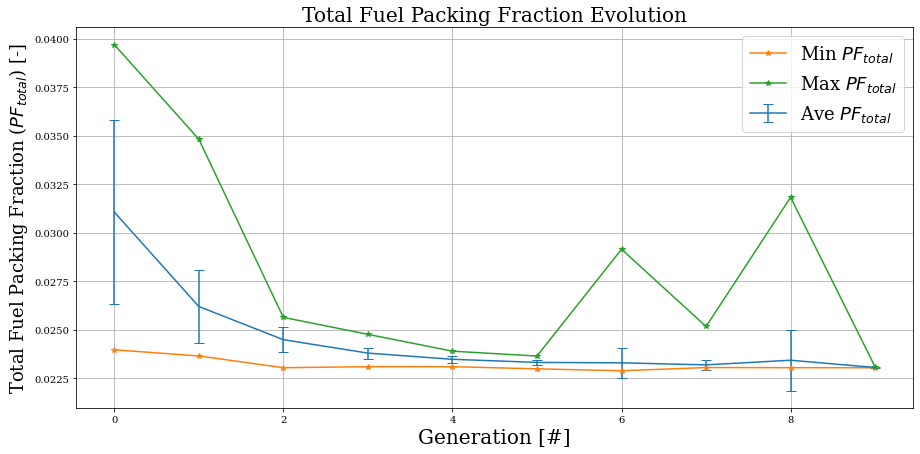
\includegraphics[width=\linewidth]{slab-obj-1-pf-evol.png}
        \caption{Minimum, average, and maximum total packing fraction evolution.}
        \label{fig:slab-obj-1-pf-evol} 
    \end{subfigure}
    \begin{subfigure}{0.95\textwidth}
        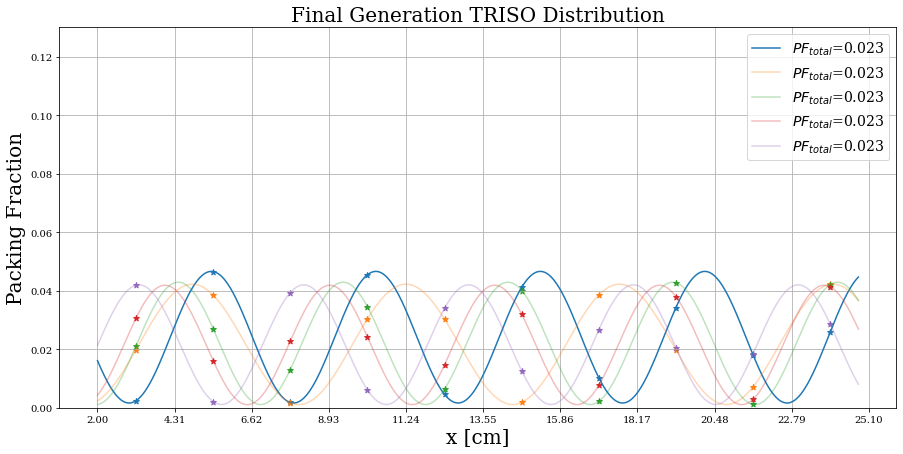
\includegraphics[width=\linewidth]{slab-obj-1-pf-final.png}
        \caption{TRISO distribution for the 5 reactor models with the 
        smallest packing fraction in the final generation.}
        \label{fig:slab-obj-1-pf-final} 
    \end{subfigure}
    \begin{subfigure}{0.95\textwidth}
        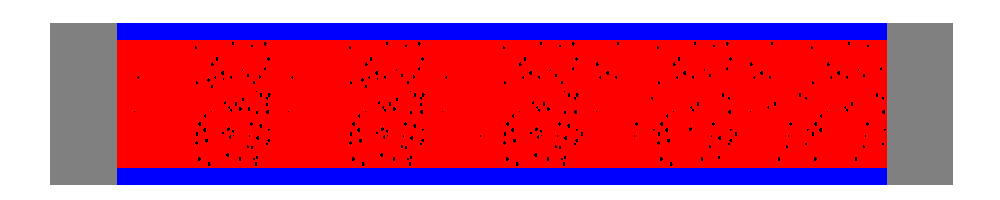
\includegraphics[width=\linewidth]{slab-obj-1-pf-most-minimized.png}
        \caption{\gls{AHTR} plank model with most-minimized total packing fraction 
        (corresponds to the blue bolded distribution in the above plot).}
        \label{fig:slab-obj-1-pf-most-minimized} 
    \end{subfigure}
    \caption{Simulation p-1a -- ROLLO single-objective optimization to minimize total 
    packing fraction. Input parameters varied: total packing fraction, TRISO particle 
    distribution.}
    \label{fig:slab-obj-1-pf}
\end{figure}

Figure \ref{fig:slab-obj-1-pf-evol} shows that the minimum and average total packing 
fraction converged very quickly, as expected in this single-objective optimization 
problem.
By the final generation, the average, minimum, and maximum packing fraction
values converged to approximately 0.023. 
In Figure \ref{fig:slab-obj-1-pf-final}, the TRISO particle packing 
sine distributions are not exactly the same, but follow a similar pattern of 
alternating between a higher packing fraction, and a lower packing fraction 
in the neighboring fuel cell. 
The oscillating fuel packing pattern minimizes self-shielding effects, enabling  
a lower packing fraction for the same $k_{eff}$. 

\subsubsection{Simulation p-1d: Variation of PF and FliBe Channel Shape}
Table \ref{tab:simulationp1d} shows simulation p-1d's optimization problem parameters. 
\begin{table}[htbp!]
    \centering
    \onehalfspacing
    \caption{Simulation p-1d Optimization Problem Parameters}
	\label{tab:simulationp1d}
    \footnotesize
    \begin{tabular}{l|p{5cm}}
    \hline 
    \multicolumn{2}{c}{\textbf{Single Objective: Simulation p-1d}} \\
    \hline 
    \textbf{Objectives} & Minimize total packing fraction\\
    \hline 
    \textbf{Input parameter variations} & $0.02<PF<0.05$ \\
    & $0.05<r_{top}<0.35$ \\
    & $0.05<r_{bot}<0.35$ \\
    \hline
    \textbf{Constraints} & $k_{eff} \geq 1.35$\\ 
    \hline 
    \textbf{Genetic algorithm parameters} & Population size: 64 \\
    & Generations: 3 \\
    \hline
    \end{tabular}
\end{table}

Figure \ref{fig:slab-obj-1-pf-evol-coolant} shows the total packing fraction evolution 
and Figure \ref{fig:slab-obj-1-pf-final-coolant} shows a plot of total radius 
($r_{top} + r_{bot}$) against total packing fraction. 
\begin{figure}[htbp!]
    \centering
    \begin{subfigure}{\textwidth}
        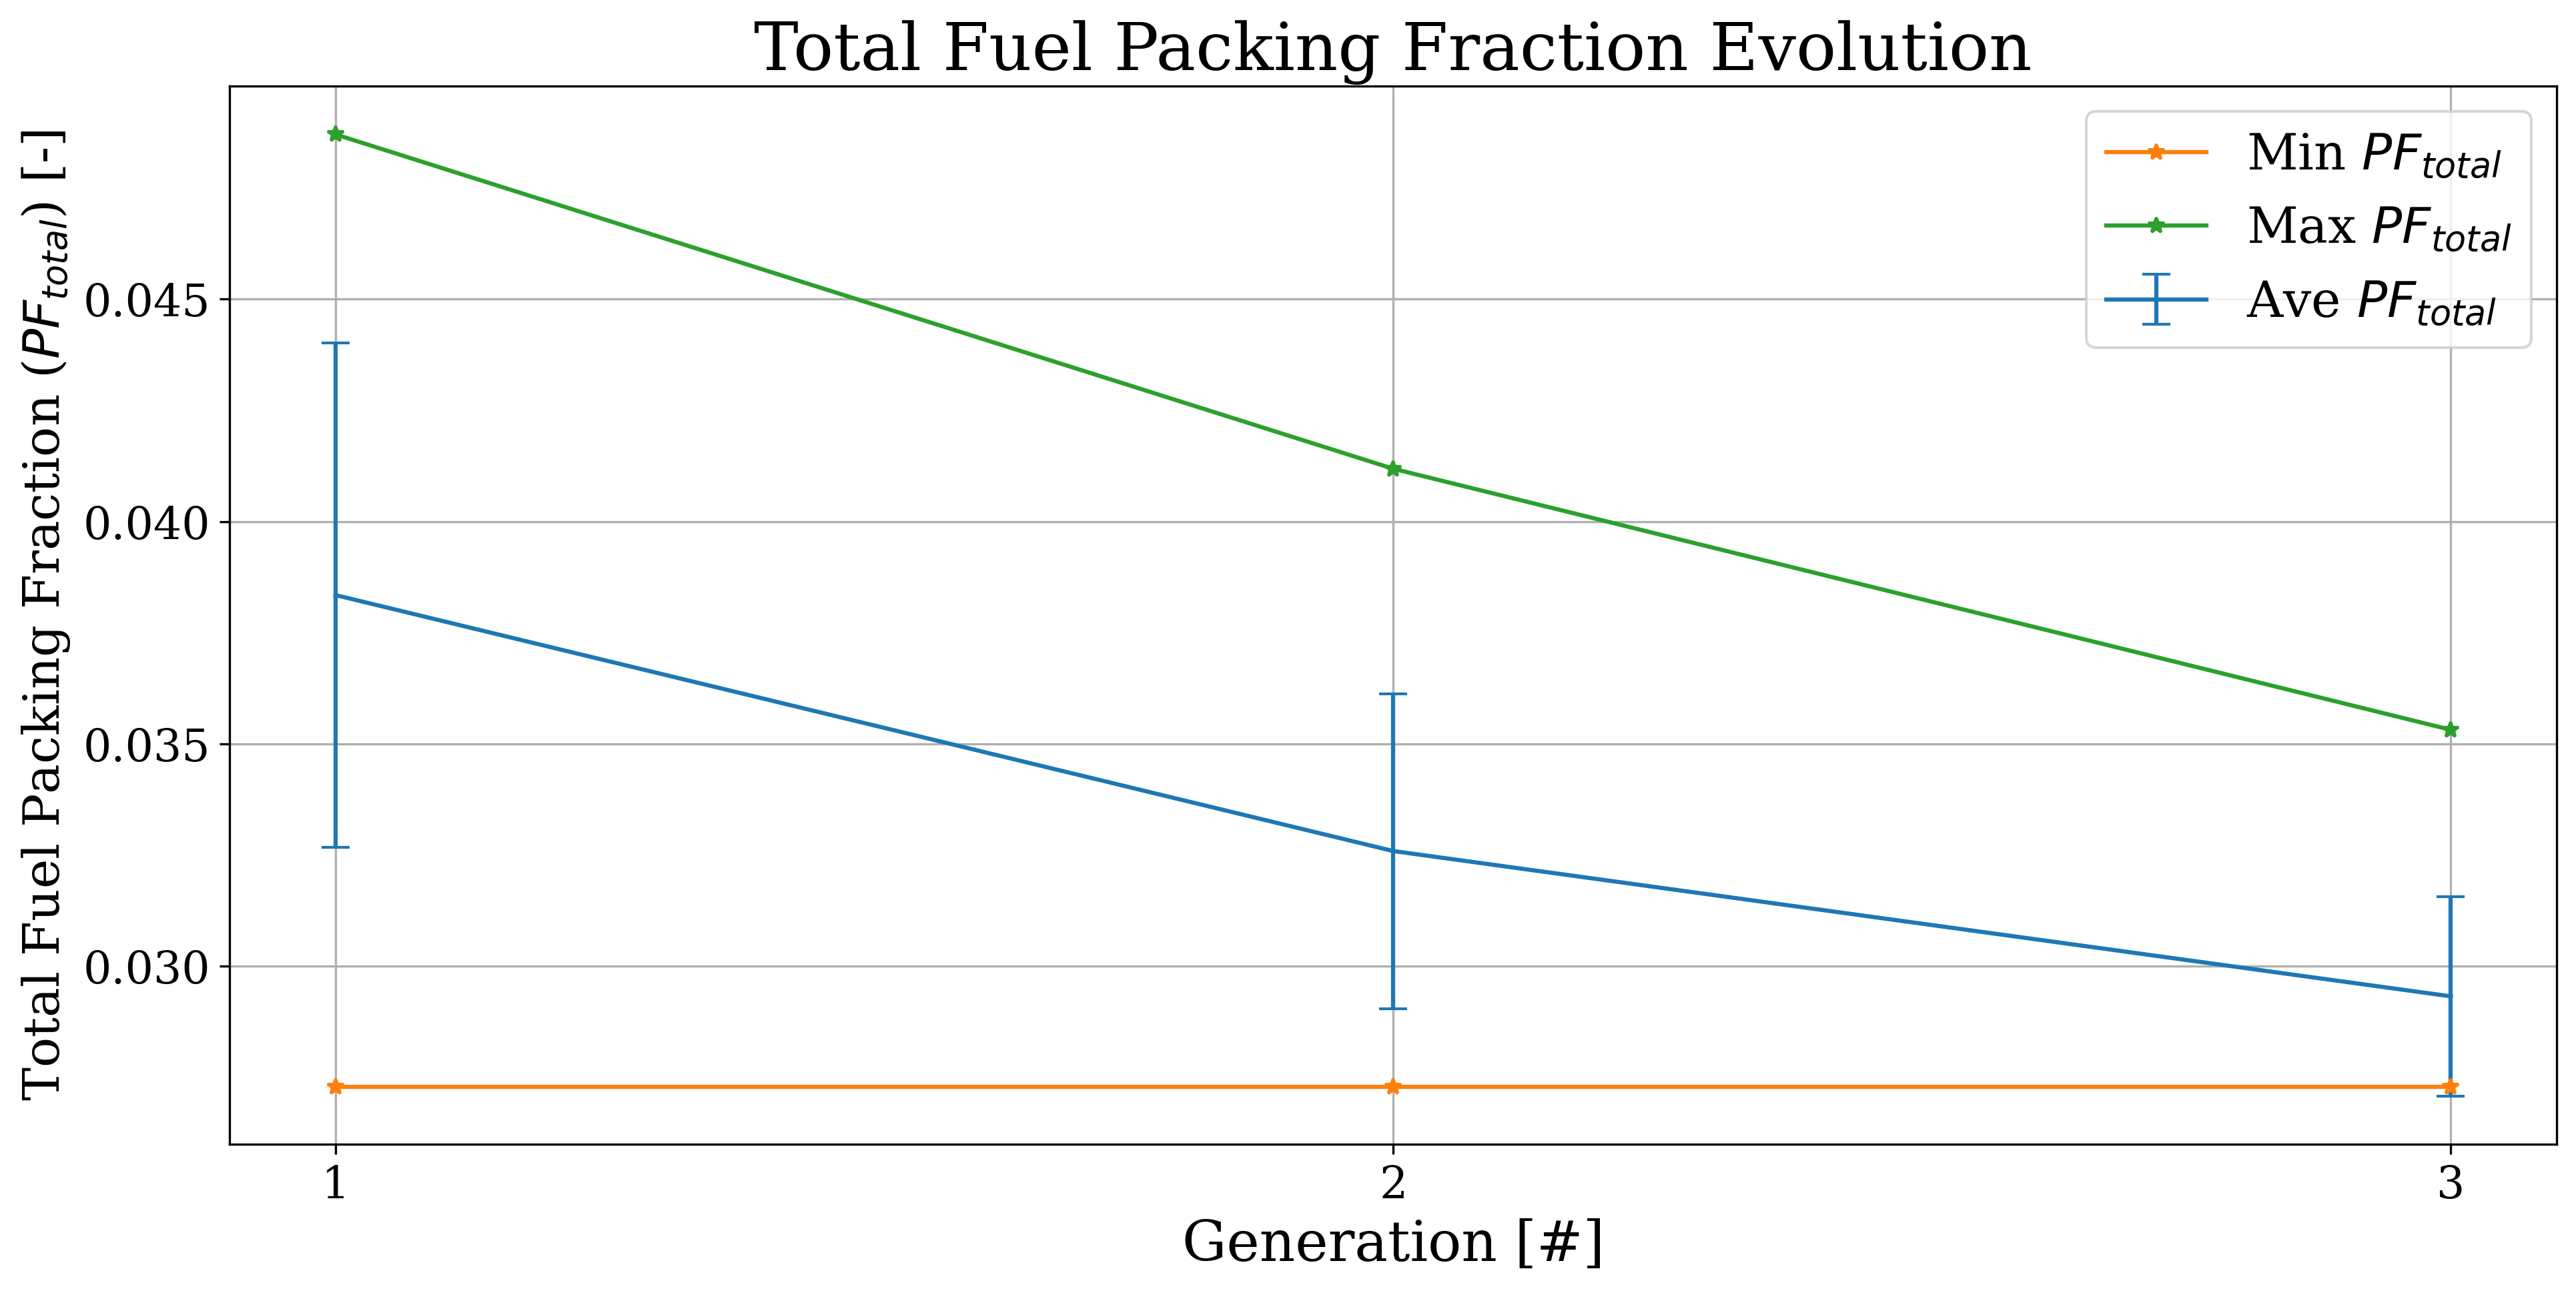
\includegraphics[width=\linewidth]{slab-obj-1-pf-evol-coolant.png}
        \caption{Minimum, average, and maximum total packing fraction evolution.}
        \label{fig:slab-obj-1-pf-evol-coolant} 
    \end{subfigure}
    \begin{subfigure}{\textwidth}
        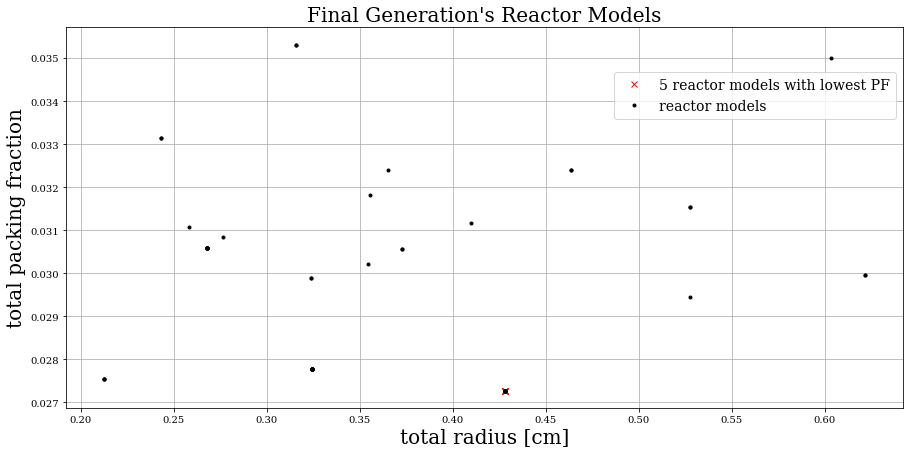
\includegraphics[width=\linewidth]{slab-obj-1-pf-final-coolant.png}
        \caption{Plot of total radius ($r_{top} + r_{bot}$) against total packing 
        fraction (PF). Red crosses indicate the five reactor models with the 
        lowest PF.}
        \label{fig:slab-obj-1-pf-final-coolant} 
    \end{subfigure}
    \caption{Simulation p-1d -- ROLLO single-objective optimization to minimize total 
    packing fraction. Input parameters varied: total packing fraction, and coolant 
    channel shape ($r_{top}, r_{bot}$).}
    \label{fig:slab-obj-1-pf-coolant}
\end{figure}
Figure \ref{fig:slab-obj-1-pf-final-coolant} demonstrates that there is no correlation 
between total packing fraction and total radius. 

\subsection{Objective: Minimize Maximum Plank Temperature ($T_{max}$)}
\label{sec:plank-1-obj-temp}
This section reports results from the minimize maximum plank temperature single-objective
optimization simulations: p-1b and p-1e. 
Simulation p-1b varies \gls{TRISO} packing fraction distribution, while simulation p-1e 
varies the \gls{FLiBe} coolant channel shape. 

\subsubsection{Simulation p-1b: Variation of $\rho_{TRISO}(\vec{r})$}
Table \ref{tab:simulationp1b} shows simulation p-1b's optimization problem parameters. 
\begin{table}[htbp!]
    \centering
    \onehalfspacing
    \caption{Simulation p-1b Optimization Problem Parameters}
	\label{tab:simulationp1b}
    \footnotesize
    \begin{tabular}{l|p{3cm}}
    \hline 
    \multicolumn{2}{c}{\textbf{Single Objective: Simulation p-1b}} \\
    \hline 
    \textbf{Objectives} & Minimize $T_{max}$ \\
    \hline 
    \textbf{Input parameter variations} & $0<a<2$ \\
    & $0<b<\frac{\pi}{2}$ \\
    & $0<c<2\pi$ \\
    \hline
    \textbf{Constraints} & $k_{eff} \geq 1.0$\\ 
    & Total PF = 0.0979\\
    \hline 
    \textbf{Genetic algorithm parameters} & Population size: 60 \\
    & Generations: 10 \\
    \hline
    \end{tabular}
\end{table}

Figure \ref{fig:slab-obj-1-temp-evol} shows the plank's $T_{max}$ evolution, Figure 
\ref{fig:slab-obj-1-temp-final} shows the five TRISO particle 
distributions in the final generation with the most-minimized $T_{max}$, and 
Figure \ref{fig:slab-obj-1-temp-most-minimized} illustrates the \gls{AHTR} plank model 
with most-minimized $T_{max}$. 
\begin{figure}[htbp!]
    \centering
    \begin{subfigure}{0.95\textwidth}
        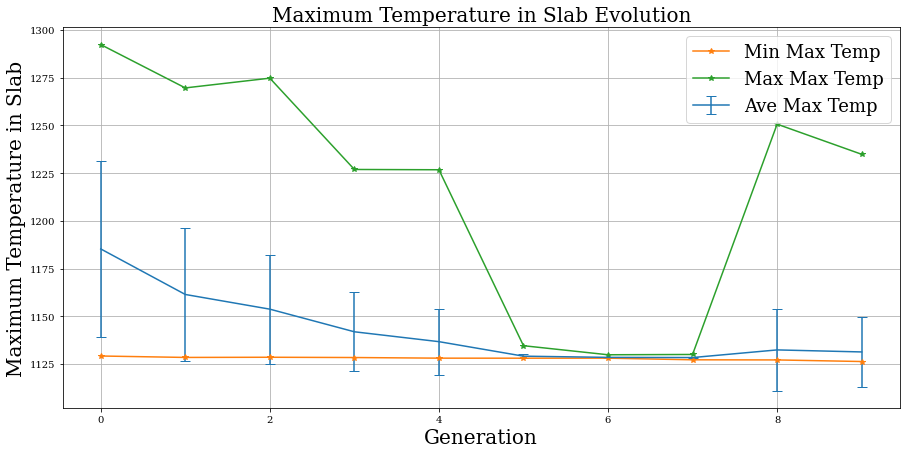
\includegraphics[width=\linewidth]{slab-obj-1-temp-evol.png}
        \caption{Minimum, average, and maximum evolution of $T_{max}$ in 
        AHTR plank.}
        \label{fig:slab-obj-1-temp-evol} 
    \end{subfigure}
    \begin{subfigure}{0.95\textwidth}
        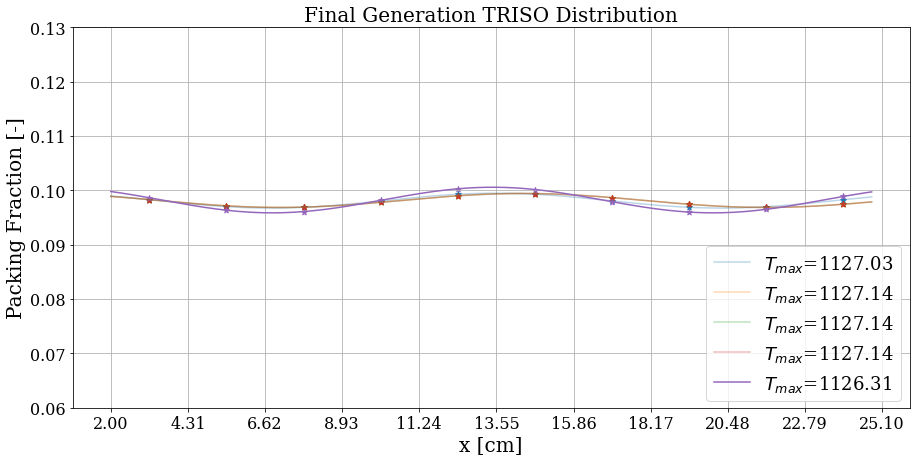
\includegraphics[width=\linewidth]{slab-obj-1-temp-final.png}
        \caption{TRISO distribution for the 5 reactor models with the 
        lowest $T_{max}$ in AHTR plank at the final generation.}
        \label{fig:slab-obj-1-temp-final} 
    \end{subfigure}
    \begin{subfigure}{0.95\textwidth}
        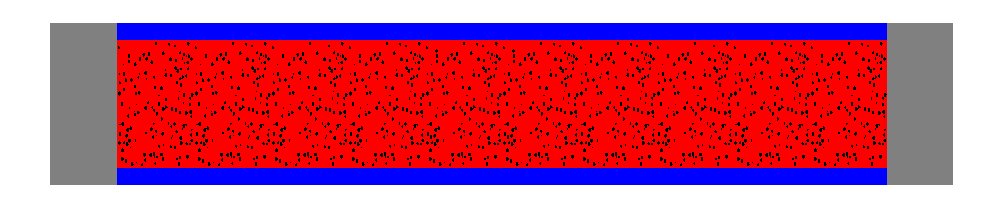
\includegraphics[width=\linewidth]{slab-obj-1-temp-most-minimized.png}
        \caption{\gls{AHTR} plank model with most-minimized $T_{max}$
        (corresponds to the purple bolded distribution in the above plot).}
        \label{fig:slab-obj-1-temp-most-minimized} 
    \end{subfigure}
    \caption{Simulation p-1b -- ROLLO single-objective optimization to minimize $T_{max}$ 
    in the plank. Input parameters varied: TRISO distribution.}
    \label{fig:slab-obj-1-temp}
\end{figure}

Figure \ref{fig:slab-obj-1-temp-evol} shows that the minimum and average plank's 
$T_{max}$ converged to approximately 1125 K. 
In Figure \ref{fig:slab-obj-1-temp-final}, a mostly flat TRISO 
particle distribution minimizes $T_{max}$ in the plank, the TRISO distribution 
has two small dips at the one-third and two-third points in the plank (6.62cm and 20.48cm). 
A fully flat \gls{TRISO} distribution results in a higher $T_{max}$.
Figure \ref{fig:slab-obj-1-temp-distr} compares the Moltres-generated centerline 
temperature distribution for the plank with mostly flat (Figure 
\ref{fig:slab-obj-1-temp-final}) and flat TRISO distributions for the same 
total packing fraction.
\begin{figure}[htbp!]
    \centering
    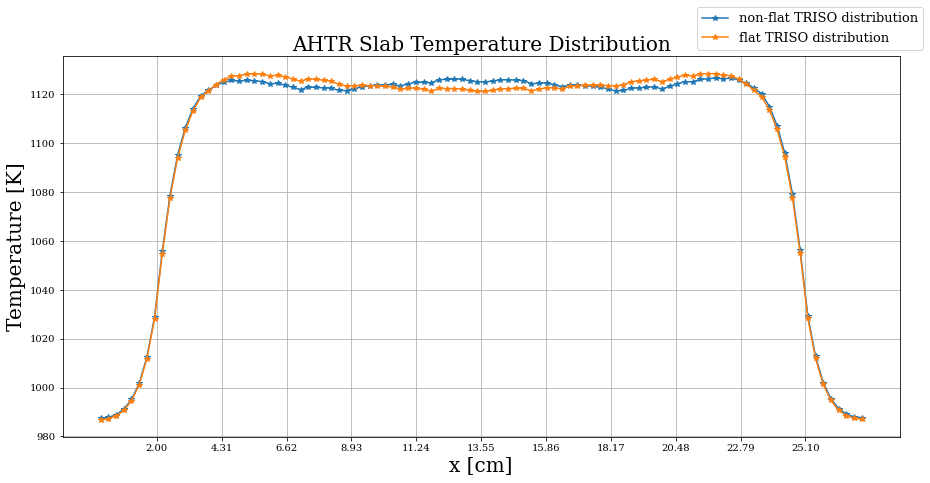
\includegraphics[width=\linewidth]{slab-obj-1-temp-distr.png}
    \caption{Comparison of Moltres-generated AHTR Plank Temperature Distribution for non-flat and flat
    TRISO distribution. Both models have a total packing fraction of 0.0979.}
    \label{fig:slab-obj-1-temp-distr}
\end{figure}
The \gls{AHTR} plank with a flat \gls{TRISO} distribution has higher plank temperatures 
on the left and right sides near the moderator. 
To combat this temperature peak, ROLLO found a \gls{TRISO} distribution that 
has a slight dip near the moderator regions, resulting in a lower $T_{max}$.

\subsubsection{Simulation p-1e: Variation of FliBe Channel Shape}
Table \ref{tab:simulationp1e} shows simulation p-1e's optimization problem parameters. 
\begin{table}[htbp!]
    \centering
    \onehalfspacing
    \caption{Simulation p-1e Optimization Problem Parameters}
	\label{tab:simulationp1e}
    \footnotesize
    \begin{tabular}{l|p{3cm}}
    \hline 
    \multicolumn{2}{c}{\textbf{Single Objective: Simulation p-1e}} \\
    \hline 
    \textbf{Objectives} & Minimize $T_{max}$ \\
    \hline 
    \textbf{Input parameter variations} & $0.05<r_{top}<0.35$ \\
    & $0.05<r_{bot}<0.35$ \\
    \hline
    \textbf{Constraints} & $k_{eff} \geq 1.35$\\ 
    & Total PF = 0.0979\\
    \hline 
    \textbf{Genetic algorithm parameters} & Population size: 64 \\
    & Generations: 4 \\
    \hline
    \end{tabular}
\end{table}

Figure \ref{fig:slab-obj-1-temp-evol-coolant} shows the plank's $T_{max}$ evolution 
and Figure \ref{fig:slab-obj-1-temp-final-coolant} shows a plot of total radius 
($r_{top} + r_{bot}$) against $T_{max}$. 
\begin{figure}[htbp!]
    \centering
    \begin{subfigure}{\textwidth}
        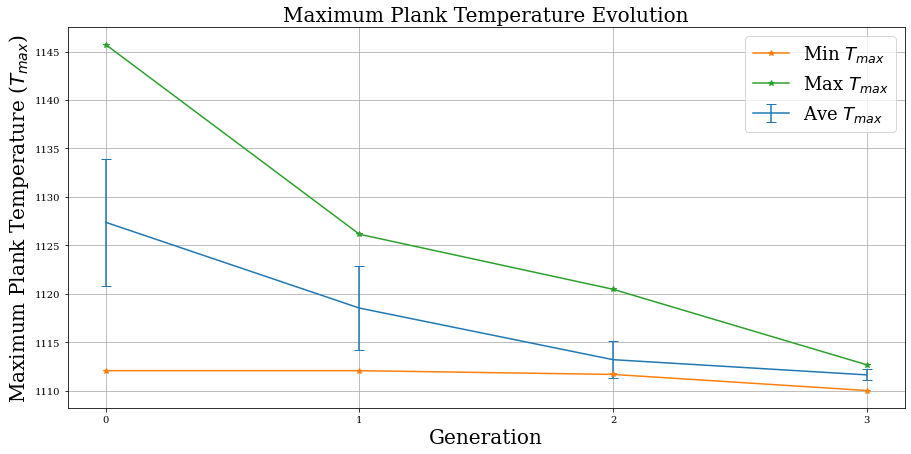
\includegraphics[width=\linewidth]{slab-obj-1-temp-evol-coolant.png}
        \caption{Minimum, average, and maximum total packing fraction evolution.}
        \label{fig:slab-obj-1-temp-evol-coolant} 
    \end{subfigure}
    \begin{subfigure}{\textwidth}
        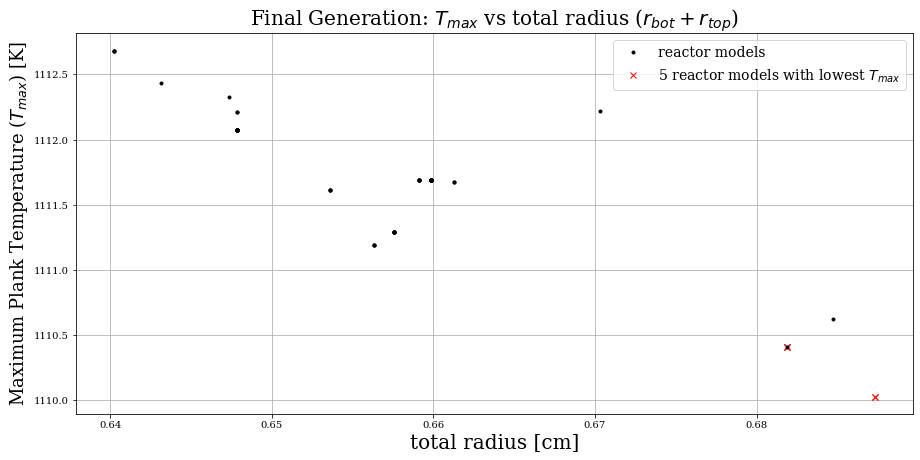
\includegraphics[width=\linewidth]{slab-obj-1-temp-final-coolant.png}
        \caption{Plot of total radius ($r_{top} + r_{bot}$) against maximum plank 
        temperature ($T_{max}$). Red crosses indicate the five reactor models with the 
        lowest $T_{max}$.}
        \label{fig:slab-obj-1-temp-final-coolant} 
    \end{subfigure}
    \caption{Simulation p-1e -- ROLLO single-objective optimization to minimize 
    maximum plank temperature ($T_{max}$). Input parameters varied: coolant channel shape 
    ($r_{top}, r_{bot}$).}
    \label{fig:slab-obj-1-temp-coolant}
\end{figure}

Figure \ref{fig:slab-obj-1-temp-final-coolant} demonstrates that there is a negative 
linear correlation between maximum plank temperature and total radius. 
Comparison of Figures \ref{fig:slab-obj-1-temp-evol} and 
\ref{fig:slab-obj-1-temp-evol-coolant} show that coolant channel shape variation 
does not have as high of an impact on $T_{max}$ as \gls{TRISO} distribution variation:  
the average $T_{max}$ due to \gls{TRISO} variation decreased by 60K over 10 generations, 
while average $T_{max}$ due to coolant channel shape variation only decreased by 15K
over 10 generations. 

\subsection{Objective: Minimize Fuel-Normalized Power Peaking Factor (PPF)}
This section reports results from the minimize fuel-normalized power peaking factor 
single-objective optimization simulations: p-1c and p-1f. 
Simulation p-1c varies \gls{TRISO} packing fraction distribution, while simulation p-1f 
varies the \gls{FLiBe} coolant channel shape. 

\subsubsection{Simulation p-1c: Variation of $\rho_{TRISO}(\vec{r})$}
Table \ref{tab:simulationp1c} shows simulation p-1c's optimization problem parameters. 
\begin{table}[htbp!]
    \centering
    \onehalfspacing
    \caption{Simulation p-1c Optimization Problem Parameters}
	\label{tab:simulationp1c}
    \footnotesize
    \begin{tabular}{l|p{3cm}}
    \hline 
    \multicolumn{2}{c}{\textbf{Single Objective: Simulation p-1c}} \\
    \hline 
    \textbf{Objectives} & Minimize PPF \\
    \hline 
    \textbf{Input parameter variations} & $0<a<2$ \\
    & $0<b<\frac{\pi}{2}$ \\
    & $0<c<2\pi$ \\
    \hline
    \textbf{Constraints} & $k_{eff} \geq 1.0$\\ 
    & Total PF = 0.0979\\
    \hline 
    \textbf{Genetic algorithm parameters} & Population size: 60 \\
    & Generations: 10 \\
    \hline
    \end{tabular}
\end{table}

Figure \ref{fig:slab-obj-1-ppf-evol} shows the plank's fuel-normalized power peaking 
factor evolution, Figure \ref{fig:slab-obj-1-ppf-final} shows the five TRISO particle 
distributions in the final generation with the most-minimized normalized power peaking 
factor, and Figure \ref{fig:slab-obj-1-ppf-most-minimized} illustrates the \gls{AHTR} 
plank model with most-minimized fuel-normalized power peaking factor. 
\begin{figure}[htbp!]
    \centering
    \begin{subfigure}{0.9\textwidth}
        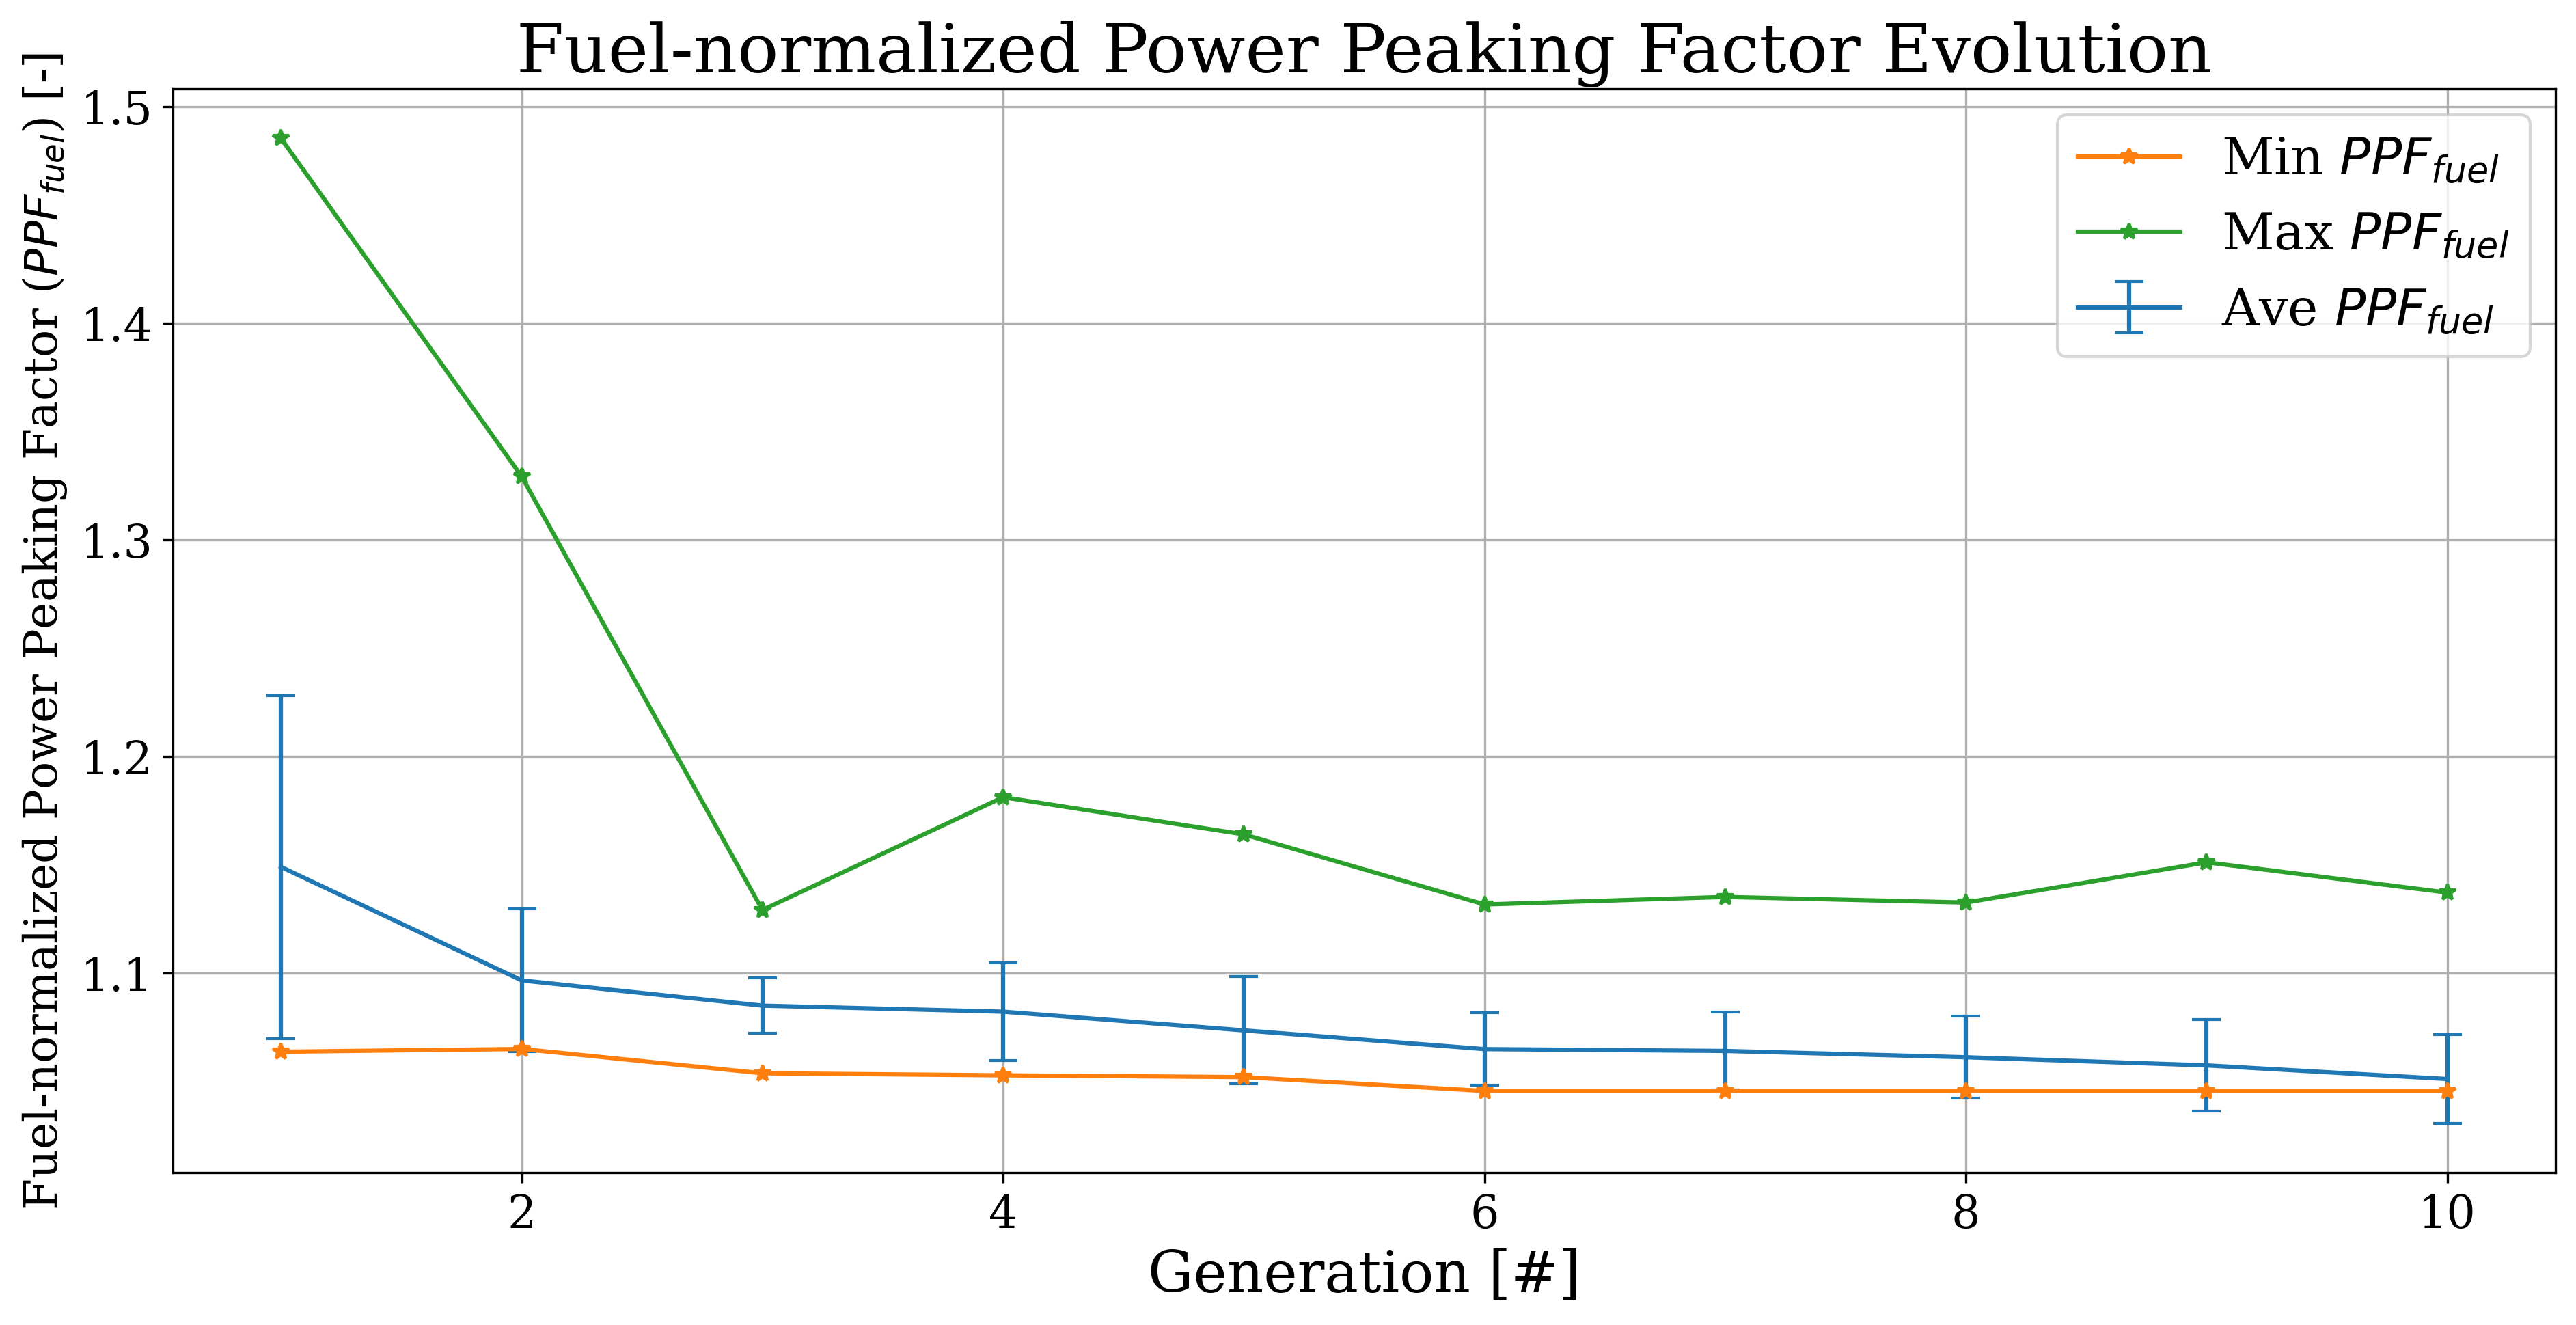
\includegraphics[width=\linewidth]{slab-obj-1-ppf-evol.png}
        \caption{Minimum, average, and maximum evolution of fuel-normalized power 
        peaking factor in AHTR slab.}
        \label{fig:slab-obj-1-ppf-evol} 
    \end{subfigure}
    \begin{subfigure}{0.9\textwidth}
        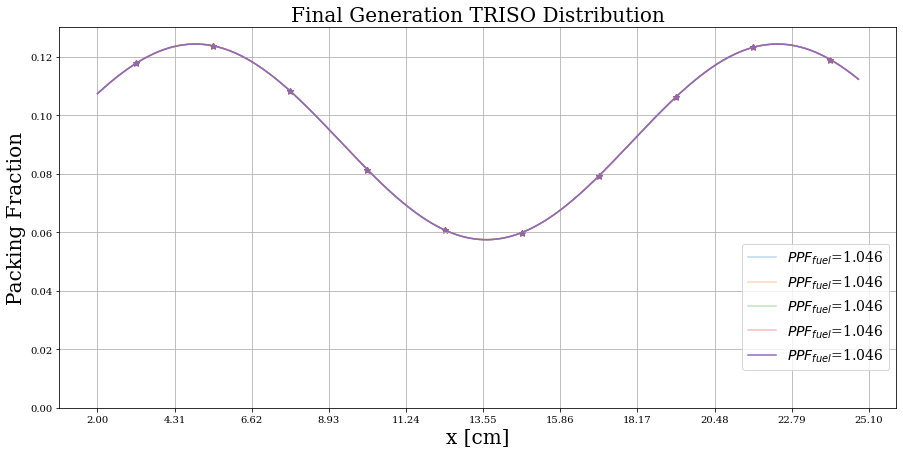
\includegraphics[width=\linewidth]{slab-obj-1-ppf-final.png}
        \caption{TRISO distribution for the 5 reactor models with the 
        lowest normalized power peaking factor in AHTR plank at the final generation.}
        \label{fig:slab-obj-1-ppf-final} 
    \end{subfigure}
    \begin{subfigure}{0.9\textwidth}
        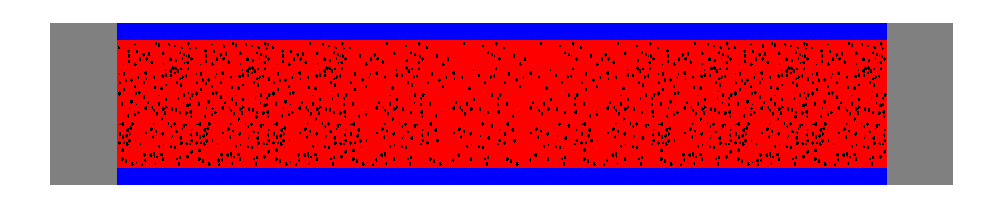
\includegraphics[width=\linewidth]{slab-obj-1-ppf-most-minimized.png}
        \caption{\gls{AHTR} plank model with most-minimized fuel-normalized power 
        peaking factor
        (corresponds to the purple bolded distribution in the above plot).}
        \label{fig:slab-obj-1-ppf-most-minimized} 
    \end{subfigure}
    \caption{Simulation p-1c -- ROLLO single-objective optimization to minimize 
    fuel-normalized power peaking factor in the plank. 
    Input parameters varied: TRISO distribution.}
    \label{fig:slab-obj-1-ppf}
\end{figure}

In Figure \ref{fig:slab-obj-1-ppf-final}, the TRISO distribution that best minimizes 
PPF peaks near the edges of the fuel region of the plank, and has a minimum point in 
center of the plank.
This distribution is attributed to the self-shielding effects. 
The edges of the fuel region have higher flux as they are closer to the graphite 
moderator, whereas the plank's center has a lower flux due to self shielding. 
Thus, to minimize fuel-normalized power peaking factor, \gls{ROLLO} found a plank 
\gls{TRISO} distribution that has higher packing fraction at the edges, and a 
lower packing fraction in the center. 

\subsubsection{Simulation p-1f: Variation of FliBe Channel Shape}
Table \ref{tab:simulationp1f} shows simulation p-1f's optimization problem parameters. 
\begin{table}[htbp!]
    \centering
    \onehalfspacing
    \caption{Simulation p-1f Optimization Problem Parameters}
	\label{tab:simulationp1f}
    \footnotesize
    \begin{tabular}{l|p{3cm}}
    \hline 
    \multicolumn{2}{c}{\textbf{Single Objective: Simulation p-1f}} \\
    \hline 
    \textbf{Objectives} & Minimize PPF \\
    \hline 
    \textbf{Input parameter variations} & $0.05<r_{top}<0.35$ \\
    & $0.05<r_{bot}<0.35$ \\
    \hline
    \textbf{Constraints} & $k_{eff} \geq 1.35$\\ 
    & Total PF = 0.0979\\
    \hline 
    \textbf{Genetic algorithm parameters} & Population size: 64 \\
    & Generations: 5 \\
    \hline
    \end{tabular}
\end{table}

Figure \ref{fig:slab-obj-1-ppf-evol-coolant} shows the plank's normalized power peaking 
factor evolution and Figure \ref{fig:slab-obj-1-ppf-final-coolant} shows a plot of total 
radius ($r_{top} + r_{bot}$) against normalized power peaking factor. 
\begin{figure}[htbp!]
    \centering
    \begin{subfigure}{\textwidth}
        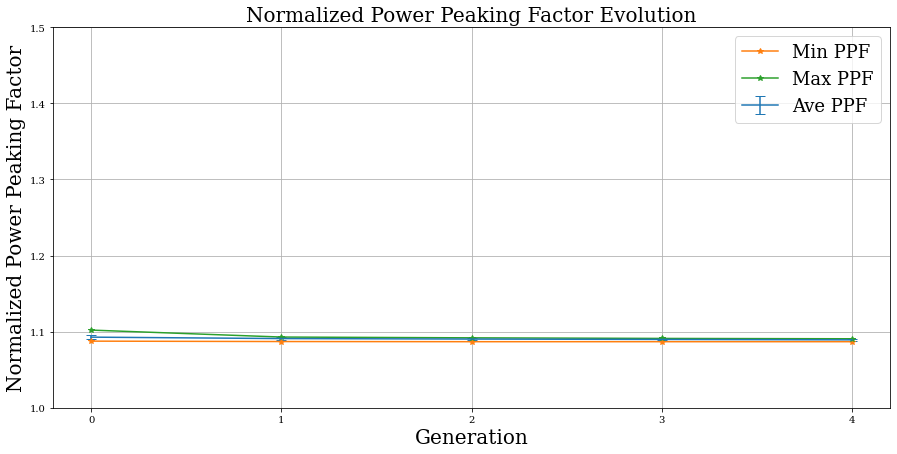
\includegraphics[width=\linewidth]{slab-obj-1-ppf-evol-coolant.png}
        \caption{Minimum, average, and maximum evolution of normalized power 
        peaking factor in AHTR plank.}
        \label{fig:slab-obj-1-ppf-evol-coolant} 
    \end{subfigure}
    \begin{subfigure}{\textwidth}
        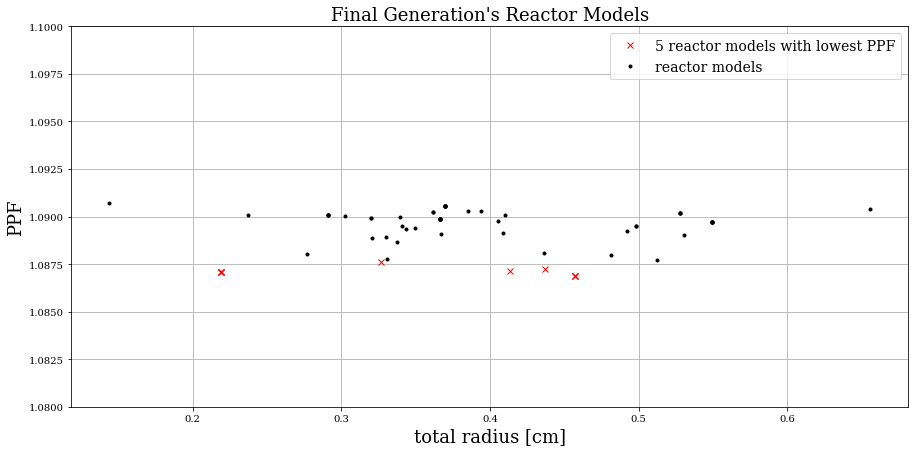
\includegraphics[width=\linewidth]{slab-obj-1-ppf-final-coolant.png}
        \caption{Plot of total radius ($r_{top} + r_{bot}$) against normalized 
        power peaking factor. Red crosses indicate the five reactor models with the 
        lowest normalized power peaking factor.}
        \label{fig:slab-obj-1-ppf-final-coolant} 
    \end{subfigure}
    \caption{Simulation p-1f -- ROLLO single-objective optimization to minimize normalized power 
    peaking factor in the slab. Input parameters varied: coolant channel shape 
    ($r_{top}, r_{bot}$).}
    \label{fig:slab-obj-1-ppf-coolant}
\end{figure}

Comparison of Figures \ref{fig:slab-obj-1-ppf-evol-coolant} and 
\ref{fig:slab-obj-1-ppf-evol} show that coolant channel shape variation 
does not have as high of an impact on PPF as \gls{TRISO} distribution variation:  
the average PPF due to \gls{TRISO} variation decreased by 0.1 over 10 generations, 
while average PPF due to coolant channel shape variation only decreased negligibly
over 10 generations. 
Figure \ref{fig:slab-obj-1-ppf-final-coolant} reiterates that there is no correlation 
between total radius and normalized power peaking factor. 

\pagebreak
\section{AHTR Plank: Two-Objective Optimization Results}
In this section, I report the \gls{AHTR} plank's \gls{ROLLO} two-objective 
optimization results. 
The previous section's one-objective optimization results inform the multi-objective 
optimization simulations.
Since the variations in coolant channel shape does not impact two out of three objectives: 
minimize total packing fraction and minimize fuel-normalized power peaking factor 
objectives, I do not conduct two-objective optimization for coolant channel shape 
variations.  
Table \ref{tab:slab-obj-breakdown} summarized the two-objective simulations in this 
section: p-2a, p-2b, and p-2c.

As previously described in Section \ref{sec:opt}, multi-objective optimization returns 
multiple optimal solutions that meet each objective to varying degrees; this set of 
solutions is the Pareto front \cite{deb_multi-objective_2001}. 
For each solution in the Pareto front, none of the objective functions can be 
improved without degrading another objective.
An ideal optimization method for a multi-objective problem like reactor design 
should find widely spread solutions in the obtained Pareto front 
\cite{deb_multi-objective_2001}. 
Thus, I report on the optimal reactor models on the Pareto front for the multi-objective 
optimization problems in this section and Section \ref{sec:plank-three-obj}. 

To ensure that the multi-objective optimization problems are converged, I report the 
hypervolume values for each generation. 
As previously described in Section \ref{sec:binhandkorn}, the hypervolume indicator 
quantifies the Pareto front's goodness (bigger = better).
I use a different reference point for each optimization problem. 
If a multi-objective optimization problem's hypervolume converges earlier than the 
5 generations I intended to run (determined in Section 
\ref{sec:multi-obj-hyperparameters}), I stop running the simulation at that generation. 

\subsection{p-2a: Minimize Total Packing Fraction and Maximum Plank Temperature}
\label{sec:p-2a}
Table \ref{tab:simulationp2a} shows simulation p-2a's optimization problem parameters. 
\begin{table}[htbp!]
    \centering
    \onehalfspacing
    \caption{Simulation p-2a Optimization Problem Parameters}
	\label{tab:simulationp2a}
    \footnotesize
    \begin{tabular}{l|p{4cm}}
    \hline 
    \multicolumn{2}{c}{\textbf{Two Objectives: Simulation p-2a}} \\
    \hline 
    \textbf{Objectives} & Minimize PF \\
    & Minimize $T_{max}$ \\
    \hline 
    \textbf{Input parameter variations} & $0.02<PF<0.04$ \\
    & $0<a<2$ \\
    & $0<b<\frac{\pi}{2}$ \\
    & $0<c<2\pi$ \\
    \hline
    \textbf{Constraints} & $k_{eff} \geq 1.35$\\ 
    \hline 
    \textbf{Genetic algorithm parameters} & Population size: 128 \\
    & Generations: 2 \\
    \hline
    \end{tabular}
\end{table}

Table \ref{tab:p2a-hypervolume} shows the hypervolume value at each generation, 
confirming that simulation p-2a converges by generation 2. 
\begin{table}[htbp!]
    \centering
    \onehalfspacing
    \caption{Simulation p-2a Hypervolume values at each generation.}
	\label{tab:p2a-hypervolume}
    \footnotesize
    \begin{tabular}{ll}
    \hline 
    \multicolumn{2}{c}{\textbf{Two Objectives: Simulation p-2a}} \\
    \multicolumn{2}{c}{Reference point: (0.1, 1350)} \\
    \hline 
    \textbf{Generation} & \textbf{Hypervolume value} \\
    \hline
    1 & 17.659 \\
    2 & 17.659 \\
    \hline
    \end{tabular}
\end{table}

Figure \ref{fig:slab-obj-2-pftemp-pareto} shows a plot of the final generation's reactor 
models' total packing fraction against $T_{max}$, crosses mark the reactor models that 
fall on the Pareto front.
Figure \ref{fig:slab-obj-2-pftemp-pareto-distr} shows the six TRISO distributions in 
the final generation that fall on the Pareto front. 
\begin{figure}[htbp!]
    \centering
    \begin{subfigure}{\textwidth}
        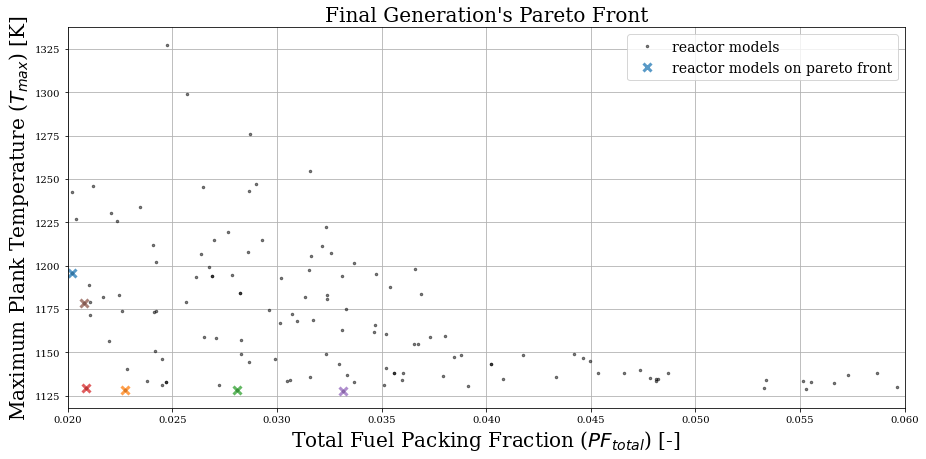
\includegraphics[width=\linewidth]{slab-obj-2-pftemp-pareto.png}
        \caption{Plot of final generation's reactor models' total packing fraction against 
        $T_{max}$. Crosses indicate the reactor models on the Pareto front. Cross colors correspond  
        to TRISO distributions in the plot below.}
        \label{fig:slab-obj-2-pftemp-pareto} 
    \end{subfigure}
    \begin{subfigure}{\textwidth}
        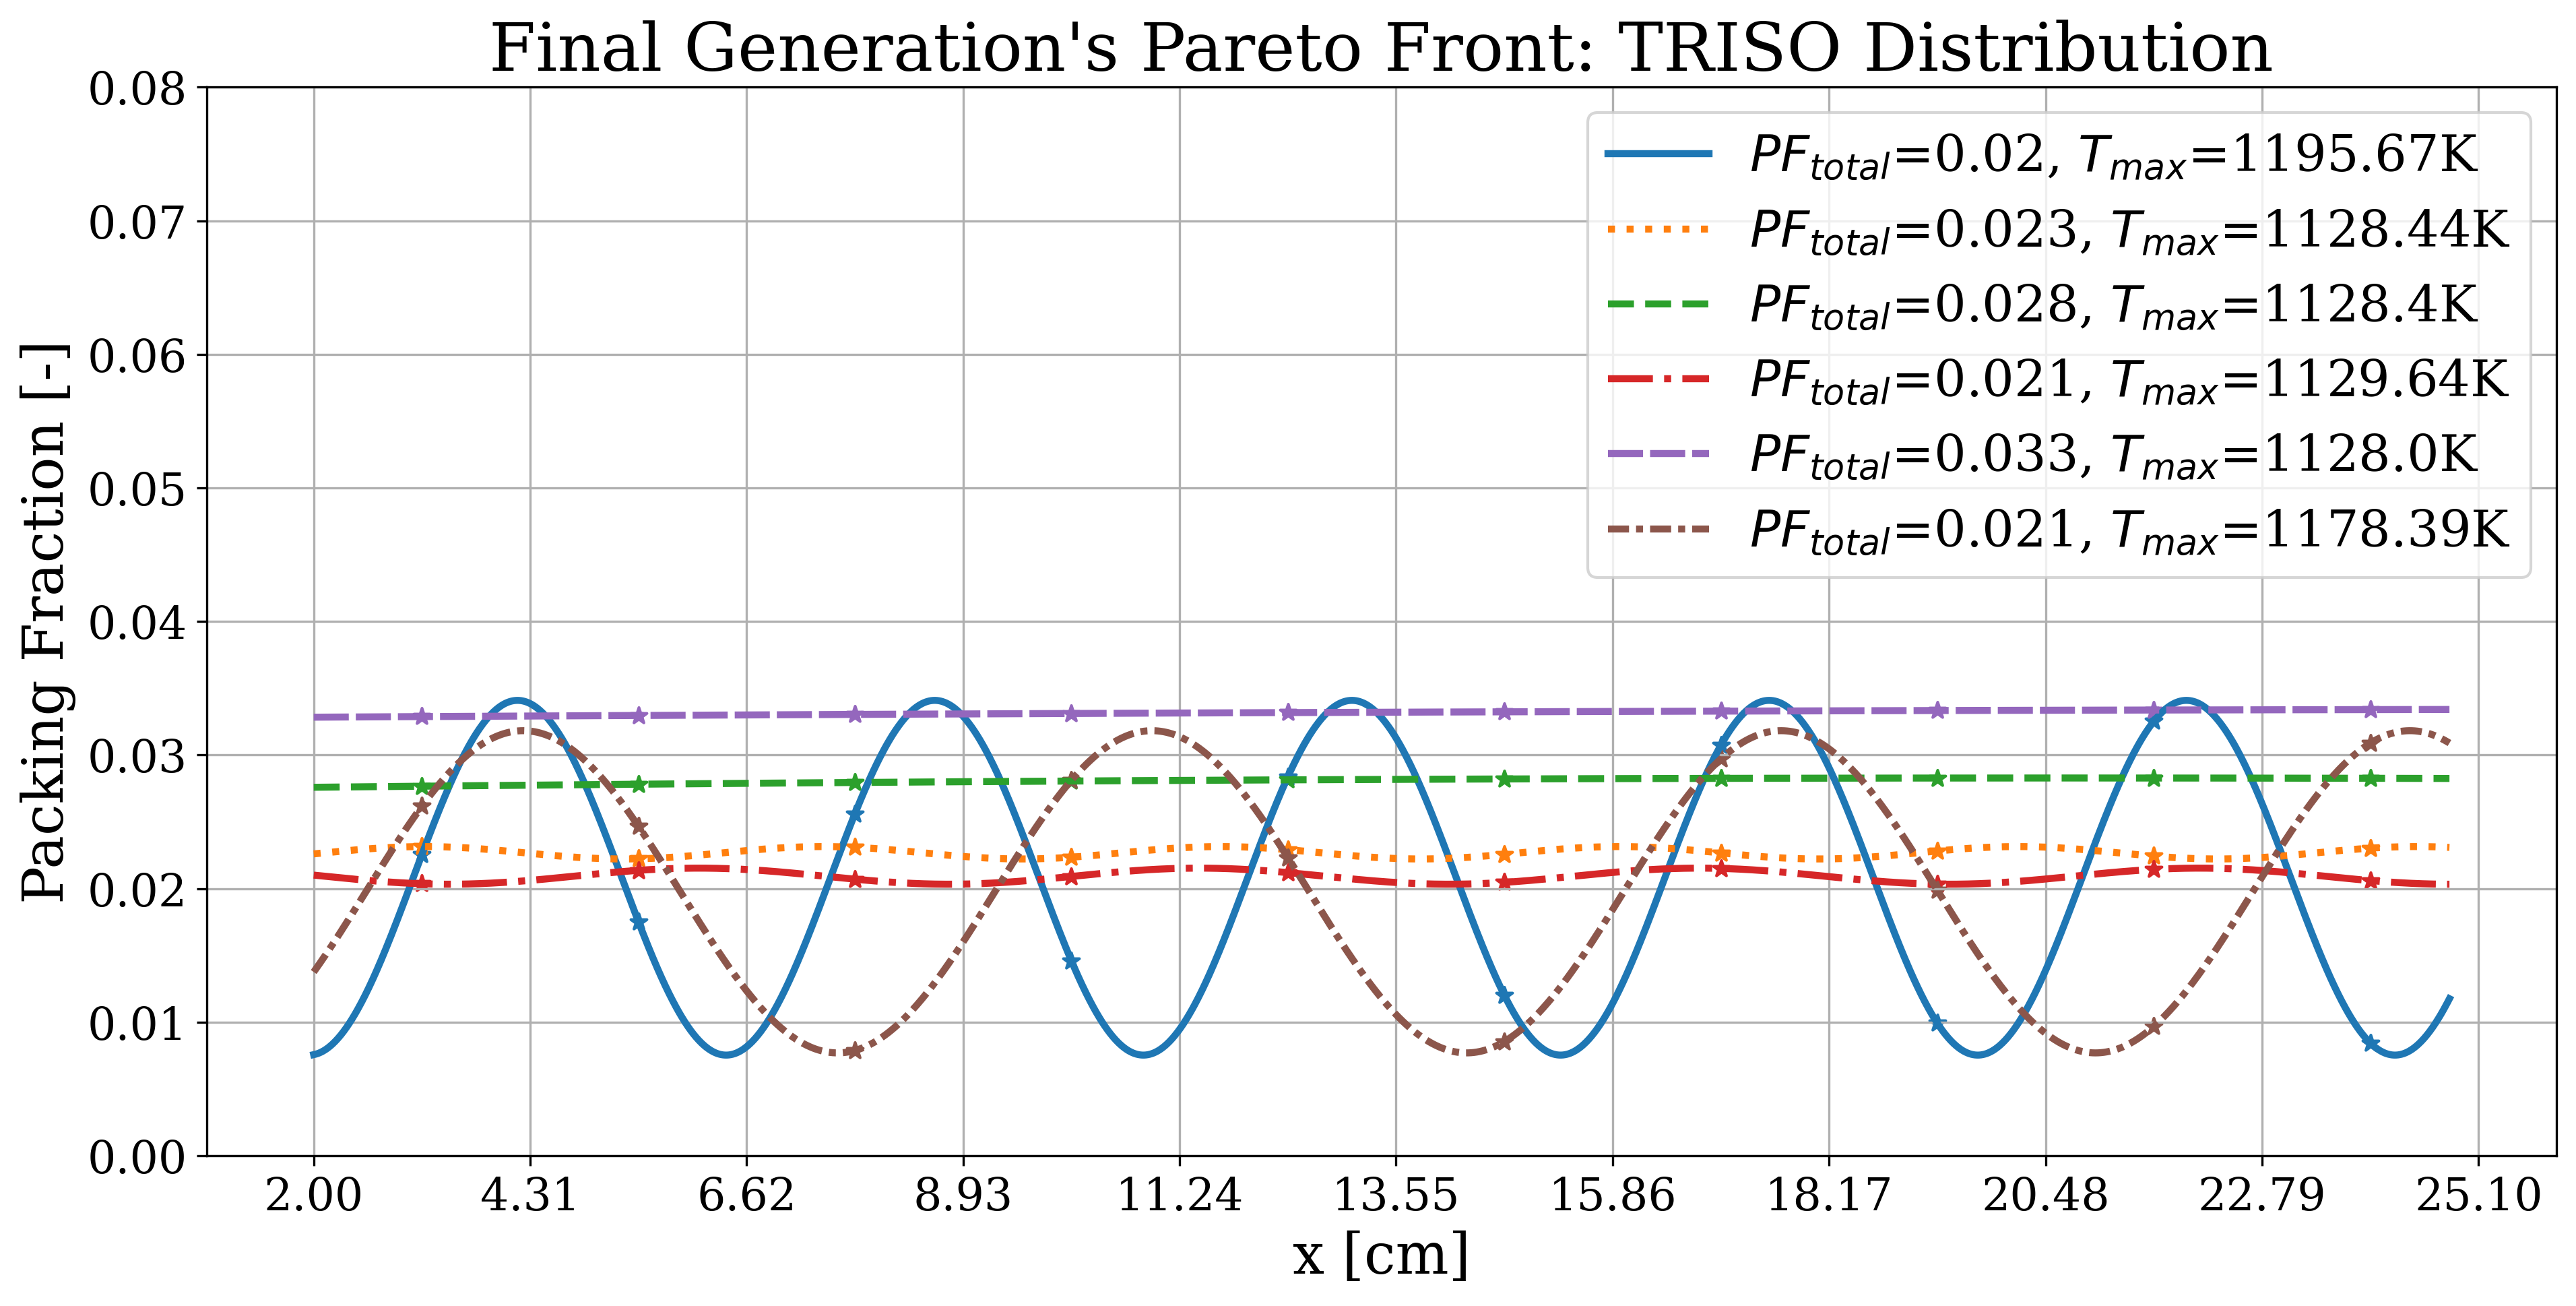
\includegraphics[width=\linewidth]{slab-obj-2-pftemp-pareto-distr.png}
        \caption{TRISO distribution for the 6 reactor models on the Pareto front.}
        \label{fig:slab-obj-2-pftemp-pareto-distr} 
    \end{subfigure}
    \caption{Simulation p-2a -- ROLLO two-objective optimization to minimize total packing fraction 
    (PF) and maximum plank temperature ($T_{max}$). 
    Input parameters varied: total fuel packing fraction and \gls{TRISO} distribution.}
    \label{fig:slab-obj-2-pftemp}
\end{figure}
\begin{figure}[htbp!]
    \ContinuedFloat
    \begin{subfigure}{\textwidth}
        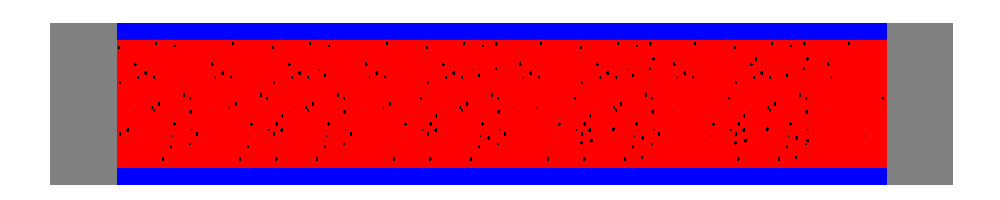
\includegraphics[width=\linewidth]{slab-obj-2-pftemp-min-pf.png}
        \caption{\gls{AHTR} plank model with most-minimized total fuel packing fraction
        (corresponds to the blue bolded distribution in Figure \ref{fig:slab-obj-2-pftemp}).}
        \label{slab-obj-2-pftemp-min-pf} 
    \end{subfigure}
    \begin{subfigure}{\textwidth}
        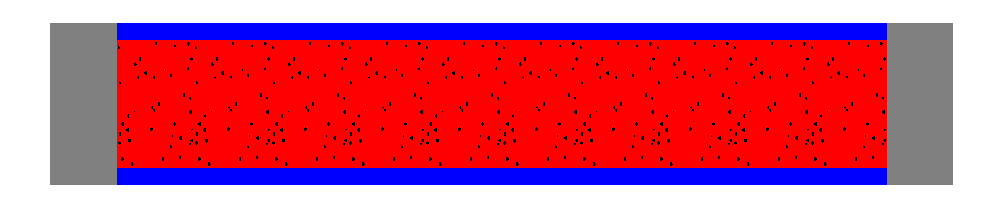
\includegraphics[width=\linewidth]{slab-obj-2-pftemp-min-temp.png}
        \caption{\gls{AHTR} plank model with most-minimized $T_{max}$
        (corresponds to the purple bolded distribution in Figure \ref{fig:slab-obj-2-pftemp}).}
        \label{slab-obj-2-pftemp-min-temp} 
    \end{subfigure}
    \caption{(contd.) Simulation p-2a -- ROLLO two-objective optimization to minimize total packing fraction 
    (PF) and maximum plank temperature ($T_{max}$). 
    Input parameters varied: total fuel packing fraction and \gls{TRISO} distribution.}
\end{figure}
In Figure \ref{fig:slab-obj-2-pftemp-pareto-distr}, the TRISO distribution with the
most-minimized total packing fraction and the highest maximum plank temperature 
(the blue distribution) has an oscillating fuel packing pattern (also illustrated in 
Figure \ref{slab-obj-2-pftemp-min-pf}).
This distribution is similar to simulation p-1a's most-minimized packing fraction TRISO 
distribution (Figure \ref{fig:slab-obj-1-pf-final}), but differs as it varies between 
0.005 and 0.035, instead of 0 and 0.4, due to influences from the minimize $T_{max}$ 
objective. 
In Figure \ref{fig:slab-obj-2-pftemp-pareto-distr}, the TRISO distribution with the 
most-minimized $T_{max}$ and highest total packing fraction (the purple distribution)
has an almost constant packing fraction of $\sim0.032$ across the plank (also 
illustrated in Figure \ref{slab-obj-2-pftemp-min-temp}). 
This distribution follows a similar flat shape as simulation p-1b's most-minimized 
$T_{max}$ TRISO distribution (Figure \ref{fig:slab-obj-1-temp-final}).

Thus, the \gls{TRISO} distributions on the Pareto front in Figure \ref{fig:slab-obj-2-pftemp} 
that minimizes both PF and $T_{max}$ have varying degrees of flatness: the minimize 
$T_{max}$ objective influences the flatness and the minimize PF objective influences 
the oscillating pattern. 

\subsection{p-2b: Minimize Total Packing Fraction and Normalized Power Peaking Factor}
Table \ref{tab:simulationp2b} shows simulation p-2b's optimization problem parameters. 
\begin{table}[htbp!]
    \centering
    \onehalfspacing
    \caption{Simulation p-2b Optimization Problem Parameters}
	\label{tab:simulationp2b}
    \footnotesize
    \begin{tabular}{l|p{3cm}}
    \hline 
    \multicolumn{2}{c}{\textbf{Two Objectives: Simulation p-2b}} \\
    \hline 
    \textbf{Objectives} & Minimize PF \\
    & Minimize PPF \\
    \hline 
    \textbf{Input parameter variations} & $0.02<PF<0.04$ \\
    & $0<a<2$ \\
    & $0<b<\frac{\pi}{2}$ \\
    & $0<c<2\pi$ \\
    \hline
    \textbf{Constraints} & $k_{eff} \geq 1.35$\\ 
    \hline 
    \textbf{Genetic algorithm parameters} & Population size: 128 \\
    & Generations: 3 \\
    \hline
    \end{tabular}
\end{table}

Table \ref{tab:p2b-hypervolume} shows the hypervolume value at each generation, 
confirming that simulation p-2b converges by generation 3. 
\begin{table}[htbp!]
    \centering
    \onehalfspacing
    \caption{Simulation p-2b Hypervolume values at each generation.}
	\label{tab:p2b-hypervolume}
    \footnotesize
    \begin{tabular}{ll}
    \hline 
    \multicolumn{2}{c}{\textbf{Two Objectives: Simulation p-2b}} \\
    \multicolumn{2}{c}{Reference point: (0.1, 1.5)} \\
    \hline 
    \textbf{Generation} & \textbf{Hypervolume value} \\
    \hline
    1 & 0.03607 \\
    2 & 0.03619 \\
    3 & 0.03625 \\
    \hline
    \end{tabular}
\end{table}

Figure \ref{fig:slab-obj-2-pfppf-pareto} shows a plot of the final generation's reactor models' 
total packing fraction against normalized power peaking factor, crosses mark the reactor 
models that fall on the Pareto front.
Figure \ref{fig:slab-obj-2-pfppf-pareto-distr} shows the four TRISO distributions in 
the final generation that fall on the Pareto front. 
\begin{figure}[htbp!]
    \centering
    \begin{subfigure}{\textwidth}
        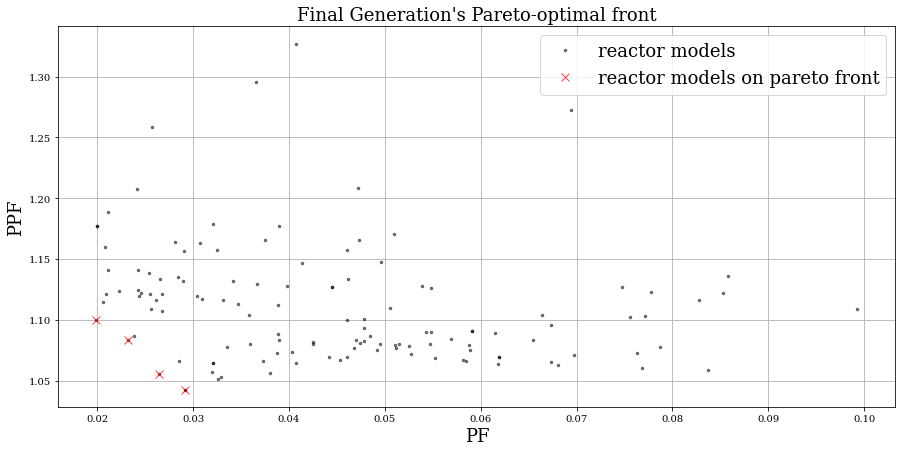
\includegraphics[width=\linewidth]{slab-obj-2-pfppf-pareto.png}
        \caption{Plot of final generation's reactor models' PF against PPF. 
        Crosses indicate the reactor models on the Pareto front. Cross colors correspond  
        to TRISO distributions in the plot below.}
        \label{fig:slab-obj-2-pfppf-pareto} 
    \end{subfigure}
    \begin{subfigure}{\textwidth}
        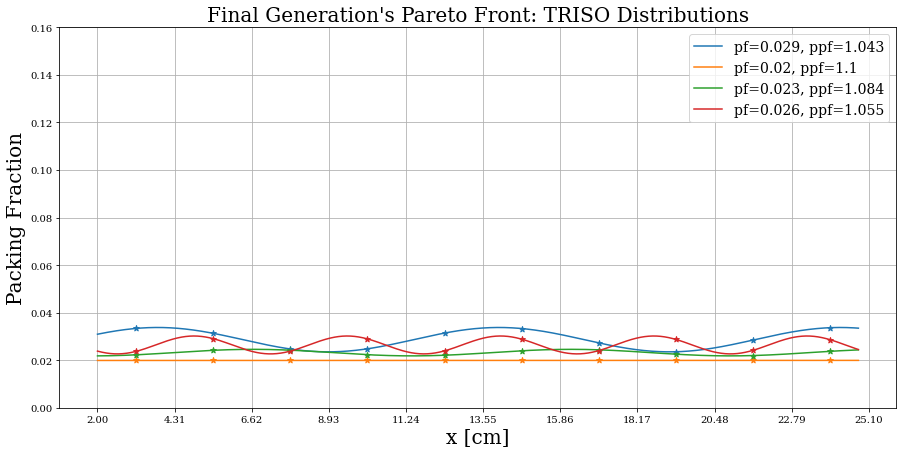
\includegraphics[width=\linewidth]{slab-obj-2-pfppf-pareto-distr.png}
        \caption{TRISO distribution for the 4 reactor models on the Pareto front.}
        \label{fig:slab-obj-2-pfppf-pareto-distr} 
    \end{subfigure}
    \caption{Simulation p-2b -- ROLLO two-objective optimization to minimize total packing 
    fraction (PF) and normalized power peaking factor (PPF) in the plank. 
    Input parameters varied: TRISO distribution.}
    \label{fig:slab-obj-2-pfppf}
\end{figure}
In Figure \ref{fig:slab-obj-2-pfppf-pareto-distr}, the TRISO distribution with the 
highest power peaking factor and lowest packing fraction (the orange distribution) has 
a constant packing fraction of 0.02 across the slab. 
In Figure \ref{fig:slab-obj-2-pfppf-pareto-distr}, the TRISO distribution with the 
lowest power peaking factor and highest packing fraction (the blue distribution), has 
a packing fraction that peaks in the center of the plank and both sides. 
All reactor models on the Pareto front have a relatively flat packing fraction 
distribution, varying between 0.02 and 0.04. 

\subsection{p-2c: Minimize Maximum Temperature and Fuel-Normalized Power Peaking Factor}
\label{sec:p-2c}
Table \ref{tab:simulationp2c} shows simulation p-2c's optimization problem parameters. 
\begin{table}[htbp!]
    \centering
    \onehalfspacing
    \caption{Simulation p-2c Optimization Problem Parameters}
	\label{tab:simulationp2c}
    \footnotesize
    \begin{tabular}{l|p{3cm}}
    \hline 
    \multicolumn{2}{c}{\textbf{Two Objectives: Simulation p-2c}} \\
    \hline 
    \textbf{Objectives} & Minimize $T_{max}$ \\
    & Minimize PPF \\
    \hline 
    \textbf{Input parameter variations} & $0<a<2$ \\
    & $0<b<\frac{\pi}{2}$ \\
    & $0<c<2\pi$ \\
    \hline
    \textbf{Constraints} & $k_{eff} \geq 1.0$\\ 
    \hline 
    \textbf{Genetic algorithm parameters} & Population size: 120 \\
    & Generations: 4 \\
    \hline
    \end{tabular}
\end{table}
Figure \ref{fig:slab-obj-2-tempppf-pareto} shows a plot of the final generation's reactor models' 
maximum plank temperature against normalized power peaking factor, crosses mark the reactor 
models that fall on the Pareto front.
Figure \ref{fig:slab-obj-2-tempppf-pareto-distr} shows the eight TRISO distributions in 
the final generation that fall on the Pareto front. 
\begin{figure}[htbp!]
    \centering
    \begin{subfigure}{\textwidth}
        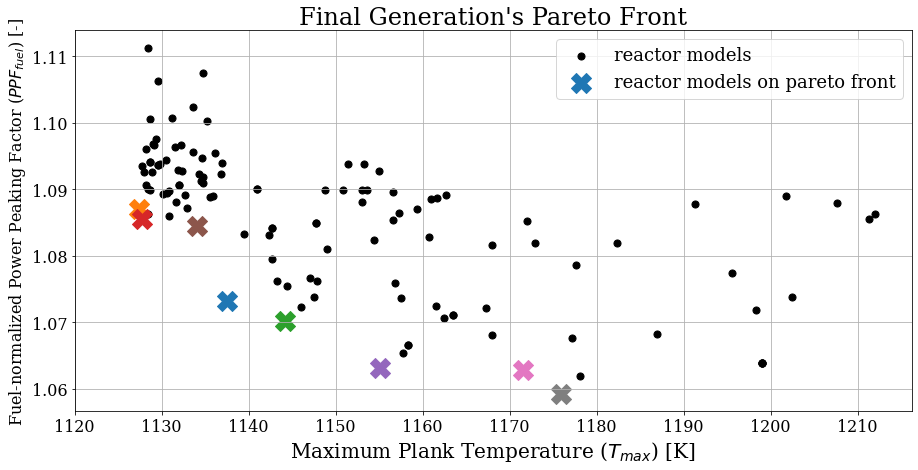
\includegraphics[width=\linewidth]{slab-obj-2-tempppf-pareto.png}
        \caption{Plot of final generation's reactor models' maximum plank temperature against normalized 
        power peaking factor. Crosses indicate the reactor models on the Pareto front. Cross colors 
        correspond to TRISO distributions in the plot below.}
        \label{fig:slab-obj-2-tempppf-pareto} 
    \end{subfigure}
    \begin{subfigure}{\textwidth}
        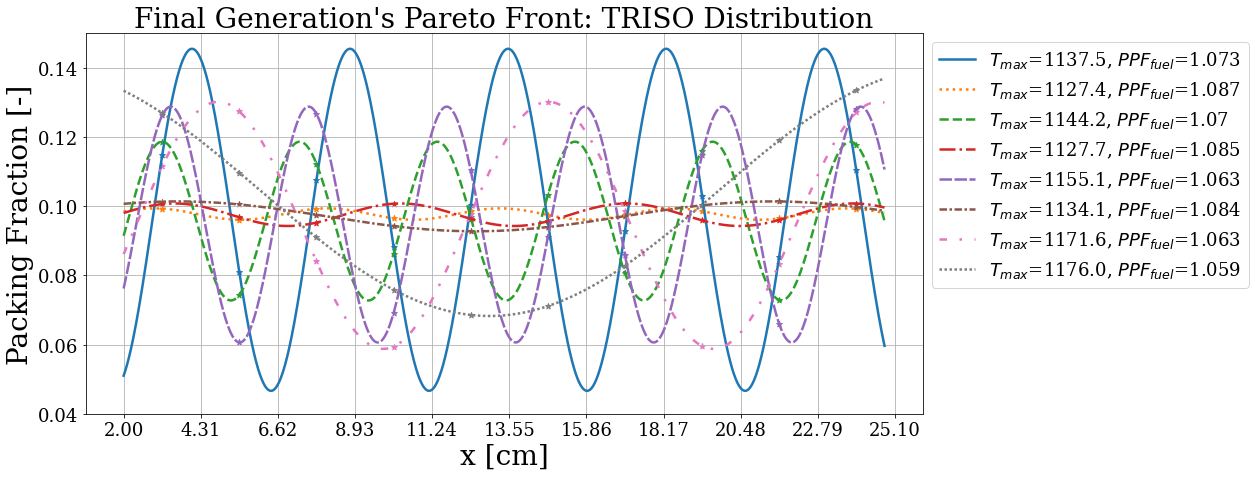
\includegraphics[width=\linewidth]{slab-obj-2-tempppf-pareto-distr.png}
        \caption{TRISO distribution for the 8 reactor models on the Pareto front.}
        \label{fig:slab-obj-2-tempppf-pareto-distr} 
    \end{subfigure}
    \caption{Simulation p-2c -- ROLLO two-objective optimization to minimize maximum plank temperature 
    ($T_{max}$) and normalized power peaking factor (PPF) in the plank. 
    Input parameters varied: TRISO distribution.}
    \label{fig:slab-obj-2-tempppf}
\end{figure}
In Figure \ref{fig:slab-obj-2-tempppf-pareto-distr}, the TRISO distribution with 
the lowest maximum temperature and highest normalized power peaking factor (the orange 
distribution) has an almost constant packing fraction of $\sim0.10$ across the slab, 
with a slight oscillating pattern. 
This distribution follows a similar flat shape as simulation p-1b's most-minimized maximum 
plank temperature TRISO distribution (Figure \ref{fig:slab-obj-1-temp-distr}).
In Figure \ref{fig:slab-obj-2-tempppf-pareto-distr}, the TRISO distribution with 
the highest maximum temperature and lowest normalized power peaking factor (the grey 
distribution) peaks near the sides of the plank, and has a minimum point at the center
of the plank. 
This distribution is somewhat similar to p-1c's most-minimized PPF TRISO distribution 
(Figure \ref{fig:slab-obj-1-ppf-final})
which also has a minimum point at the center of the plank, but differs as its' peaks 
are on the fuel regions' edges instead of the plank's edges. 

The differences between the above cases and their single objective counterparts are due to 
influences from the other objectives. 

\pagebreak
\section{AHTR Plank: Three-Objective Optimization Results}
\label{sec:plank-three-obj}

\subsection{p-3a: Variation of of $\rho_{TRISO}(\vec{r})$ and Total Packing Fraction}
Table \ref{tab:simulationp3a} shows simulation p-3a's optimization problem parameters. 
\begin{table}[htbp!]
    \centering
    \onehalfspacing
    \caption{Simulation p-3a Optimization Problem Parameters}
	\label{tab:simulationp3a}
    \footnotesize
    \begin{tabular}{l|p{4cm}}
    \hline 
    \multicolumn{2}{c}{\textbf{Three Objectives: Simulation p-3a}} \\
    \hline 
    \textbf{Objectives} & Minimize PF \\
    & Minimize $T_{max}$ \\
    & Minimize PPF \\
    \hline 
    \textbf{Input parameter variations} & $0.02<PF<0.04$ \\
    & $0<a<2$ \\
    & $0<b<\frac{\pi}{2}$ \\
    & $0<c<2\pi$ \\
    \hline
    \textbf{Constraints} & $k_{eff} \geq 1.35$\\ 
    \hline 
    \textbf{Genetic algorithm parameters} & Population size: 128 \\
    & Generations: 5 \\
    \hline
    \end{tabular}
\end{table}

Figure \ref{fig:slab-obj-3-3d} shows a 3D plot of the final generation's reactor models' 
total packing fraction against maximum plank temperature against normalized power 
peaking factor, crosses mark the reactor models that fall on the Pareto front.
Figure \ref{fig:slab-obj-3-distr} shows the 14 TRISO distributions in 
the final generation that fall on the Pareto front. 
\begin{figure}[htbp!]
    \begin{subfigure}{\textwidth}
        \centering
        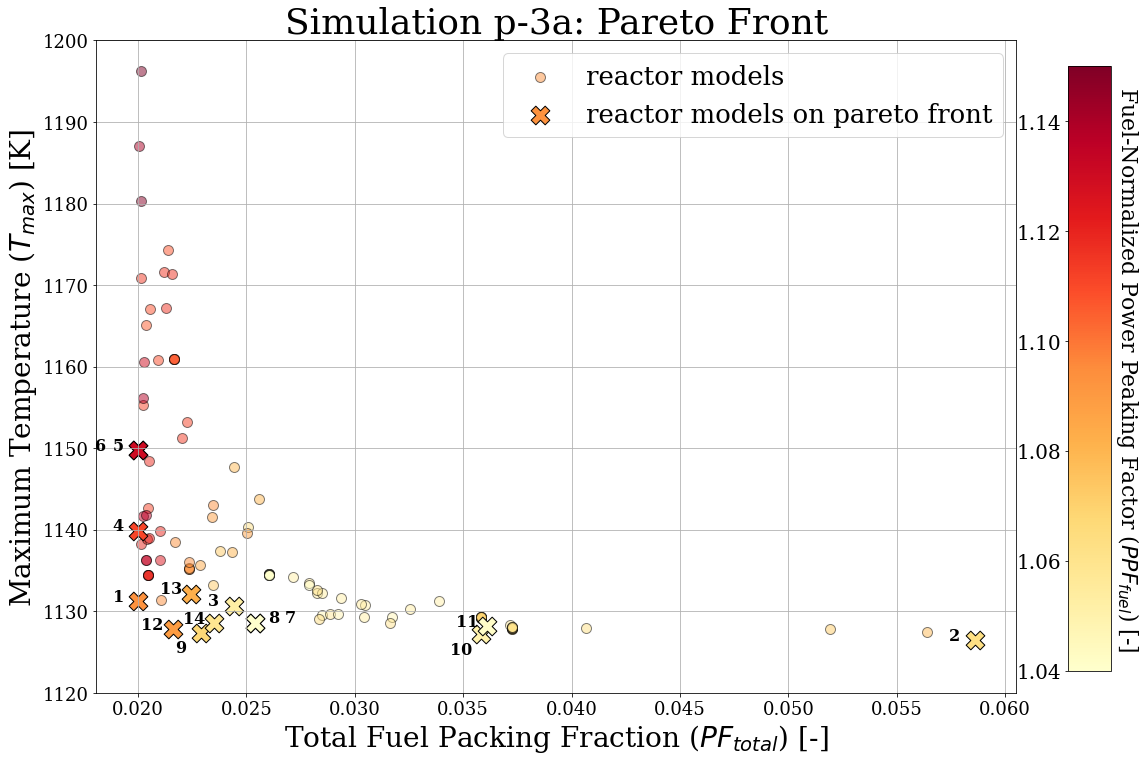
\includegraphics[width=0.7\linewidth]{slab-obj-3-3d.png}
        \caption{Plot of final generation's reactor models' total packing fraction against maximum plank 
        temperature against normalized power peaking factor. Crosses indicate the reactor models on the 
        Pareto front. Cross colors correspond to TRISO distributions in the plot below.}
        \label{fig:slab-obj-3-3d} 
    \end{subfigure}
    \begin{subfigure}{\textwidth}
        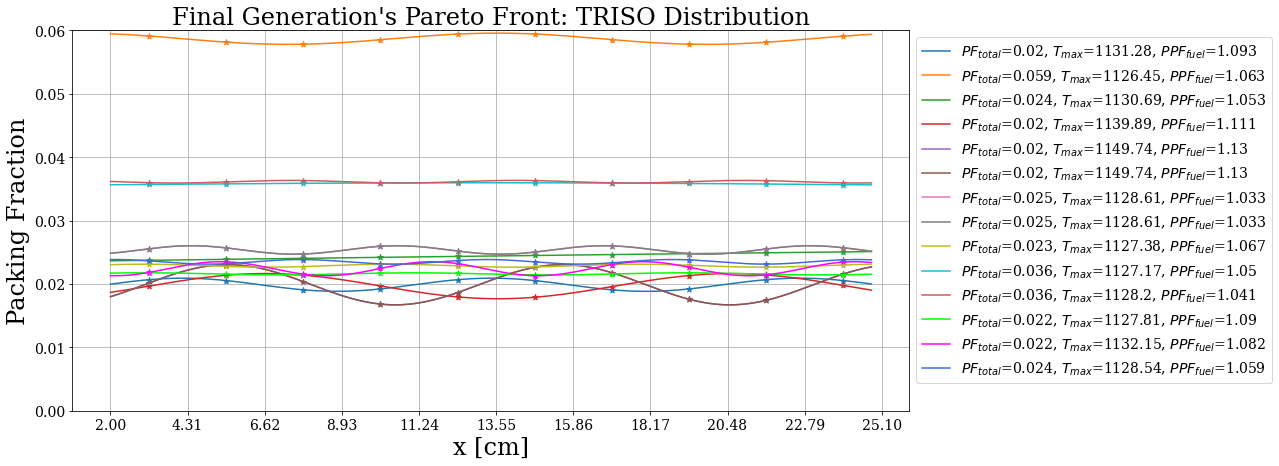
\includegraphics[width=\linewidth]{slab-obj-3-distr.png}
        \caption{TRISO distribution for the 14 reactor models on the Pareto front.}
        \label{fig:slab-obj-3-distr} 
    \end{subfigure}
    \caption{Simulation p-3a -- ROLLO three-objective optimization to minimize total packing fraction, 
    maximum plank temperature ($T_{max}$) and normalized power peaking factor (PPF) in the plank. 
    Input parameters varied: Total PF, TRISO distribution.}
    \label{fig:slab-obj-3}
\end{figure}

Figure \ref{fig:slab-obj-3-3d} demonstrates that \gls{ROLLO} found 14 widely spread 
solutions in the final generation's Pareto front. 
Figure \ref{fig:slab-obj-3-distr} demonstrates that the TRISO distributions on the
Pareto front have maximum packing fraction variation of $\sim0.01$. 
Figure \ref{fig:slab-obj-3-distr-most-minimized} shows the three distributions from 
Figure \ref{fig:slab-obj-3-distr} that most-minimized each objective. 
\begin{figure}[htbp!]
    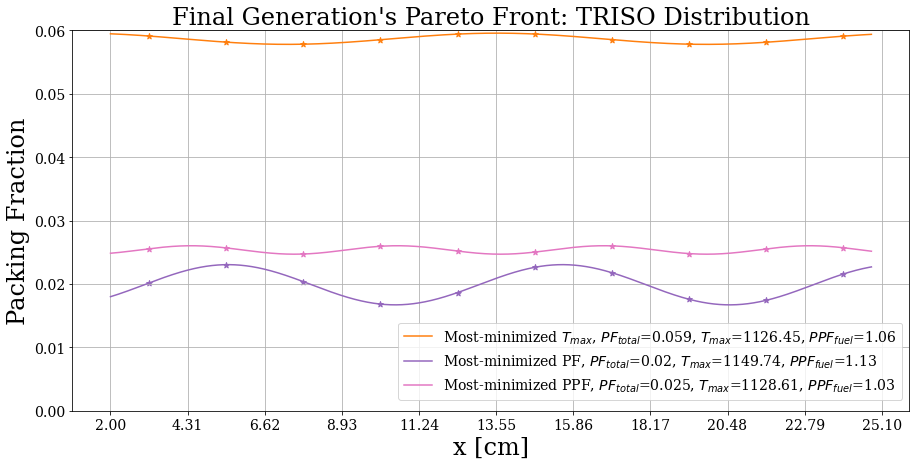
\includegraphics[width=\linewidth]{slab-obj-3-distr-most-minimized.png}
    \caption{Simulation p-3a -- ROLLO three-objective optimization to minimize total packing fraction, 
    maximum plank temperature ($T_{max}$) and normalized power peaking factor (PPF) in the plank. 
    Input parameters varied: TRISO distribution. TRISO distribution for the 3 reactor models on the Pareto front
    that most minimized each objective.}
    \label{fig:slab-obj-3-distr-most-minimized}
\end{figure}
The brown distribution with oscillating fuel packing pattern most-minimized total packing fraction. 
The blue distribution with a mostly flat fuel distribution most-minimized $T_{max}$. 
The grey distribution with small oscillating fuel packing pattern most-minimized normalized 
power peaking factor. 

\subsection{p-3b: Variation of $\rho_{TRISO}(\vec{r})$, Total Packing Fraction, and FliBe Channel Shape}
Table \ref{tab:simulationp3b} shows simulation p-3b's optimization problem parameters. 
\begin{table}[htbp!]
    \centering
    \onehalfspacing
    \caption{Simulation p-3b Optimization Problem Parameters}
	\label{tab:simulationp3b}
    \footnotesize
    \begin{tabular}{l|p{4cm}}
    \hline 
    \multicolumn{2}{c}{\textbf{Three Objectives: Simulation p-3b}} \\
    \hline 
    \textbf{Objectives} & Minimize PF \\
    & Minimize $T_{max}$ \\
    & Minimize PPF \\
    \hline 
    \textbf{Input parameter variations} & $0.02<PF<0.04$ \\
    & $0<a<2$ \\
    & $0<b<\frac{\pi}{2}$ \\
    & $0<c<2\pi$ \\
    & $0.05<r_{top}<0.35$ \\
    & $0.05<r_{bot}<0.35$ \\
    \hline
    \textbf{Constraints} & $k_{eff} \geq 1.35$\\ 
    \hline 
    \textbf{Genetic algorithm parameters} & Population size: 128 \\
    & Generations: 5 \\
    \hline
    \end{tabular}
\end{table}

Figure \ref{fig:slab-obj-3-3d-all} shows a 3D plot of the final generation's reactor 
models' total packing fraction against maximum plank temperature against normalized
power peaking factor, crosses mark the reactor models that fall on the Pareto front.
Figure \ref{fig:slab-obj-3-distr-all} shows the 13 TRISO distributions and their
total radius $(r_{top}, r_{bot})$ in the final generation that fall on the Pareto 
front. 
\begin{figure}[htbp!]
    \begin{subfigure}{\textwidth}
        \centering
        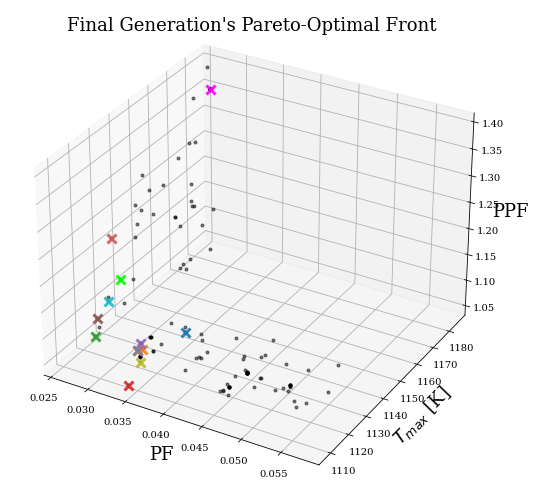
\includegraphics[width=0.7\linewidth]{slab-obj-3-3d-all.png}
        \caption{Plot of final generation's reactor models' total packing fraction against maximum plank 
        temperature against normalized power peaking factor. Crosses indicate the reactor models on the 
        Pareto front. Cross colors correspond to TRISO distributions in the plot below.}
        \label{fig:slab-obj-3-3d-all} 
    \end{subfigure}
    \begin{subfigure}{\textwidth}
        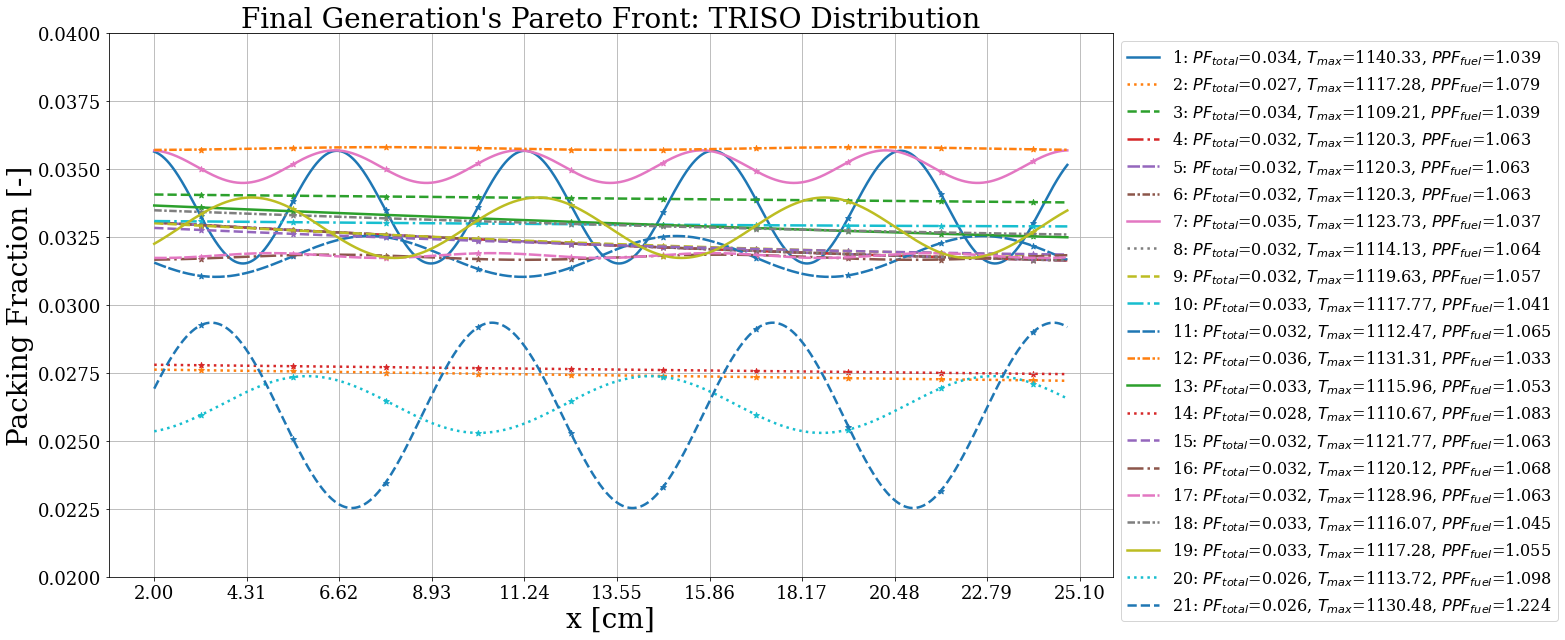
\includegraphics[width=\linewidth]{slab-obj-3-distr-all.png}
        \caption{TRISO distribution for the 13 reactor models on the Pareto front.}
        \label{fig:slab-obj-3-distr-all} 
    \end{subfigure}
    \caption{Simulation p-3b -- ROLLO three-objective optimization to minimize total packing fraction, 
    maximum plank temperature ($T_{max}$) and normalized power peaking factor (PPF) in the plank. 
    Input parameters varied: Total PF, TRISO distribution, 
    coolant channel shape $(r_{top}, r_{bot})$.}
    \label{fig:slab-obj-3-all}
\end{figure}

Figure \ref{fig:slab-obj-3-3d-all} demonstrates that \gls{ROLLO} found 13 widely spread 
solutions in the final generation's Pareto front. 
Figure \ref{fig:slab-obj-3-distr-most-minimized-distr-all} shows the three distributions 
from Figure \ref{fig:slab-obj-3-distr-all} that most-minimized each objective. 
Figures \ref{fig:slab-obj-3-distr-most-minimized-pf-all}, \ref{fig:slab-obj-3-distr-most-minimized-temp-all}, 
and \ref{fig:slab-obj-3-distr-most-minimized-ppf-all} show the \gls{AHTR} plank's TRISO 
distribution and coolant channel shape for most-minimized cases. 
\begin{figure}[htbp!]
    \begin{subfigure}{\textwidth}
        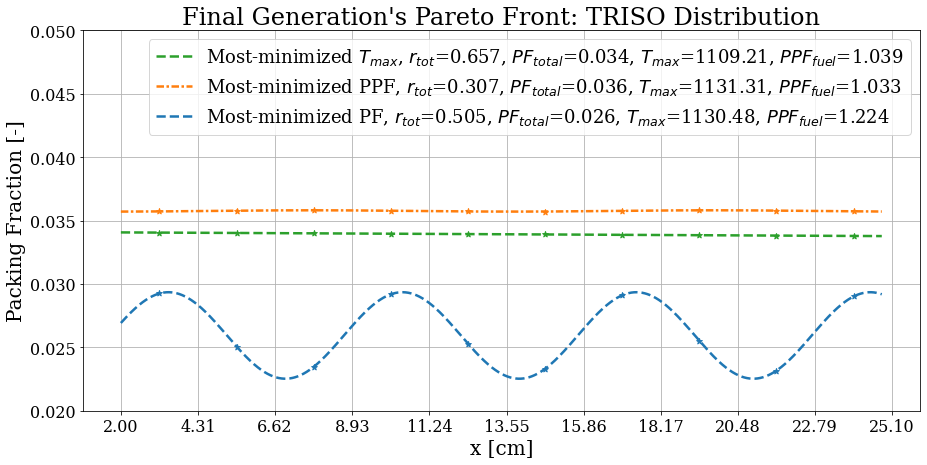
\includegraphics[width=\linewidth]{slab-obj-3-distr-most-minimized-all.png}
        \caption{TRISO distribution for the 3 reactor models on the Pareto 
        front that most minimized each objective.}
        \label{fig:slab-obj-3-distr-most-minimized-distr-all}
    \end{subfigure}
    \begin{subfigure}{\textwidth}
        
\includegraphics[width=\linewidth]{plank-pf-min-4-1.png}
        \caption{TRISO distribution and coolant channel shape that most minimized Total 
        PF (green distribution).}
        \label{fig:slab-obj-3-distr-most-minimized-pf-all}
    \end{subfigure}
    \begin{subfigure}{\textwidth}
        
\includegraphics[width=\linewidth]{plank-temp-min-3-17.png}
        \caption{TRISO distribution and coolant channel shape that most minimized 
        $T_{max}$ (brown distribution).}
        \label{fig:slab-obj-3-distr-most-minimized-temp-all}
    \end{subfigure}
    \begin{subfigure}{\textwidth}
        
\includegraphics[width=\linewidth]{plank-ppf-min-1-42.png}
        \caption{TRISO distribution and coolant channel shape that most minimized PPF
        (blue distribution).}
        \label{fig:slab-obj-3-distr-most-minimized-ppf-all}
    \end{subfigure}
    \caption{Simulation p-3b -- ROLLO three-objective optimization to minimize total 
    packing fraction, maximum plank temperature ($T_{max}$) and normalized power peaking 
    factor (PPF) in the plank. 
    Input parameters varied: Total PF, TRISO distribution, and coolant channel shape 
    $(r_{top}, r_{bot})$.}
    \label{fig:slab-obj-3-distr-most-minimized-all}
\end{figure}
The green distribution with sloping fuel packing distribution and $r_{tot} = 0.385cm$ 
most-minimized total packing fraction. 
The brown distribution with a mostly flat fuel distribution and $r_{tot} = 0.584cm$ 
most-minimized $T_{max}$. 
The blue distribution with small oscillating fuel packing pattern and $r_{tot} = 0.193cm$ 
most-minimized normalized power peaking factor. 

Most of the \gls{TRISO} distributions on the Pareto front have a mostly flat 
distribution with approximately $\sim0.1cm$ of variation. 
The flatness is influenced by the minimize $T_{max}$ objective. 
As observed in previous sections \ref{sec:plank-1-obj-temp}, \ref{sec:p-2a}, and 
\ref{sec:p-2c}, a flat \gls{TRISO} distribution minimizes $T_{max}$ objective.
The variations in \gls{TRISO} distributions are influenced by both the minimize 
total packing fraction and minimize PPF objectives. 
The minimize total packing fraction objective tries to minimize self shielding effects 
to enable a higher $k_{eff}$ for lower total PF. 
The minimize fuel-normalized power peaking factor objective tries to minimize 
TRISO distribution in areas with higher flux to minimize fuel-normalized power peaking.
% talk about coolant channel shape influences T_max. but not as much 
% the other objectives are not impacted by coolant channel shape. 

Section \ref{sec:plank-discussion} gives further discussion on \gls{ROLLO}'s plank 
optimization results and significance for reactor designers.

\pagebreak
\section{AHTR Plank: Computational Cost Summary}
\label{sec:plank-compute-cost}
Simulations are run on the BlueWaters supercomputer \cite{ncsa_about_2017} and Theta 
supercomputer at the Argonne Leadership Computing Facility under the Director's 
Discretionary Allocation Program \cite{noauthor_argonne_2022}. 
Each optimization problem takes a different amount of node-hours to run due to 
differences in simulation software, tallies and intermediate steps required. 

Table \ref{tab:plank-compute-cost} reports the computational cost for each optimization 
problem. 
Table \ref{tab:slab-obj-breakdown} details the simulation parameters. 
%The BW supercomputer uses 32 nodes 
% Theta specs ... 
\begin{table}[htbp!]
    \centering
    \onehalfspacing
    \caption{Computational cost of \acrfull{ROLLO} simulations for optimizing \acrfull{AHTR}
    plank.}
	\label{tab:plank-compute-cost}
    \footnotesize
    \begin{tabular}{p{1.4cm}|p{1cm}lp{4cm}lp{4cm}}
    \hline 
    \textbf{Num of Objs} & \textbf{Sim} & \textbf{Machine} & \textbf{Compute cost per gen [node-hours]} &\textbf{gens} & \textbf{Total compute cost [node-hours]} \\
    \hline
    \multirow{6}{2cm}{1} 
    & p-1a & BW & 23.8 & 10 & 238.6\\
    & p-1b & BW & 95.9 & 10 & 959.6\\
    & p-1c & & & & \\
    & p-1d & Theta & 49.5 & 3 & 148.7\\
    & p-1e & Theta & 71.4 & 4 & 285.6\\
    & p-1f & Theta & 82.7 & 5 & 413.8 \\
    \hline
    \multirow{3}{2cm}{2}
    & p-2a & Theta & 87.6 & 2 & 175.2\\
    & p-2b & Theta & & 3 & \\
    & p-2c & Theta & & & \\
    \hline
    \multirow{2}{2cm}{3}
    & p-3a & Theta & & & \\
    & p-3b & Theta & & & \\
    \hline
    \end{tabular}
\end{table}

\section{AHTR Plank Optimization Results Discussion and Significance}
\label{sec:plank-discussion}
\gls{ROLLO} successfully finds widely spread solutions in each of the multi-objective 
optimization final generation's Pareto front.
\gls{ROLLO} is a global search of a large design space and helps narrow down possible 
solutions.
This informs reactor designers of optimal reactor parameters for their defined objectives.  
From here, reactor designers can conduct sensitivity analysis and use high fidelity 
models to characterize a smaller section of the design space.

\section{Summary}